%convert -coalesce launch.gif launch_%d.png
\documentclass{beamer}

\newcommand{\VEV}[1]{\langle#1\rangle}
\newcommand{\sst}{\left(1-\frac{2M}{r}\right)}
\newcommand{\sh}{\mathrm{shell}}
\newcommand{\be}{\begin{equation}}
\newcommand{\ee}{\end{equation}}
\newcommand{\bue}{\begin{equation}}
\newcommand{\eue}{\end{equation}}
\newcommand{\bc}{\begin{center}}
\newcommand{\ec}{\end{center}}
\newcommand{\bea}[1]{\begin{eqnarray}\label{#1}}
\newcommand{\eea}{\end{eqnarray}}
\newcommand{\bua}{\begin{eqnarray*}}
\newcommand{\eua}{\end{eqnarray*}}
\newcommand{\dd}[2]{{{d#1}\over{d#2}}}
\newcommand{\ddt}[1]{\dd{#1}{t}}
\newcommand{\dddt}[1]{\dd{^2#1}{t^2}}
\newcommand{\aver}[1]{\langle{#1}\rangle}
\newcommand{\atom}[3]{\ifmmode^{#1}_{#2}{\rm{#3}}\else{$^{#1}_{#2}${#3}}\fi}
\newcommand{\electron}{\atom{~0}{-1}{e}}
\newcommand{\positron}{\atom{0}{0}{\bar{e}}}
\newcommand{\neutrino}{\atom{0}{0}{\nu_e}}
\newcommand{\photon}{\atom{0}{0}{\gamma}}
\newcommand{\antineutrino}{\atom{0}{0}{\bar{\nu}}}
\newcommand{\neutron}{\atom{1}{0}{n}}
\newcommand{\proton}{\atom{1}{1}{p}}
\newcommand{\hydrogen}{\atom{1}{1}{H}}
\newcommand{\deuterium}{\atom{2}{1}{H}}
\newcommand{\tritium}{\atom{3}{1}{H}}
\newcommand{\helium}{\atom{4}{2}{He}}
\newcommand{\hethree}{\atom{3}{2}{He}}

\renewcommand{\ss}{Schwarz\-schild }

\def\densu{kg/m$^3$} 
\def\rsol{R$_{\odot}$} 
\def\msol{M$_{\odot}$} 

\newcommand{\htmlcom}[1]{\^#1\^}


\usetheme{Boadilla}
%\usepackage{multimedia}
%\usepackage{animate}
\usepackage{hyperref}
\usepackage{tikz}
\usepackage{cancel}
\usepackage{tikzsymbols}
\usepackage{ifthen}

%%%%mathcircled
\makeatletter
\newcommand\mathcircled[1]{%`
  \mathpalette\@mathcircled{#1}%
}
\newcommand\@mathcircled[2]{%
  \tikz[baseline=(math.base)] \node[draw,circle,red, thick, inner sep=2pt] (math) {$\m@th#1#2$};%
}
\makeatother
%%%%

%gets rid of bottom navigation bars
\setbeamertemplate{footline}[frame number]{}

%gets rid of bottom navigation symbols
\setbeamertemplate{navigation symbols}{}

%gets rid of footer
%will override 'frame number' instruction above
%comment out to revert to previous/default definitions
\setbeamertemplate{footline}{}

\definecolor{darkscarlet}{rgb}{0.34, 0.01, 0.1}
\definecolor{gold(metallic)}{rgb}{0.83, 0.69, 0.22}
\definecolor{green(ryb)}{rgb}{0.4, 0.69, 0.2}
\definecolor{darkorange}{rgb}{1.0, 0.55, 0.0}
\definecolor{amber}{rgb}{1.0, 0.75, 0.0}
\definecolor{bronze}{rgb}{0.8, 0.5, 0.2}
\definecolor{cadet}{rgb}{0.33, 0.41, 0.47}
\definecolor{silver}{rgb}{0.75, 0.75, 0.75}
\definecolor{turquoise}{rgb}{0.19, 0.84, 0.78}
\definecolor{uclagold}{rgb}{1.0, 0.7, 0.0}
\definecolor{urobilin}{rgb}{0.88, 0.68, 0.13}
\definecolor{vegasgold}{rgb}{0.77, 0.7, 0.35}
\definecolor{vanilla}{rgb}{0.95, 0.9, 0.67}
\definecolor{straw}{rgb}{0.89, 0.85, 0.44}
\definecolor{sunset}{rgb}{0.98, 0.84, 0.65}
\definecolor{brown(traditional)}{rgb}{0.59, 0.29, 0.0}
\definecolor{apricot}{rgb}{0.98, 0.81, 0.69}
\definecolor{darkblue}{rgb}{0,0,0.54}

\hypersetup{
    colorlinks=true,
    linkcolor=yellow,
    filecolor=magenta,      
    urlcolor=blue,
}

\let\hrefori\href
\renewcommand{\href}[2]{{\setlength{\fboxsep}{1pt}\colorbox{sunset}{\hrefori{#1}{#2}}}}


%title
\setbeamercolor{block title alerted}{fg=white,bg=cyan}
%body
\setbeamercolor{block body alerted}{fg=black!90,bg=yellow!60}

%title
\setbeamercolor{block title}{fg=black,bg=turquoise}
%body
\setbeamercolor{block body}{fg=yellow,bg=bronze}




\newcommand{\pagebutton}[1]{\setbeamertemplate{button}{\tikz\node[inner xsep = 5pt, draw = structure!90, fill = green(ryb), rounded corners = 8pt]{\color{amber}\Large\insertbuttontext};}\beamerbutton{#1}}

\newcommand{\choicebutton}[1]{\setbeamertemplate{button}{\tikz\node[inner xsep = 8pt, draw = structure!90, fill = vegasgold, rounded corners = 5pt]{\color{vanilla}\Large\insertbuttontext};}\beamerbutton{#1}}

\newcommand{\pagenobutton}[1]{\setbeamertemplate{button}{\tikz\node[inner xsep = 8pt, draw = structure!90, fill = apricot, rounded corners = 5pt]{\color{brown(traditional)}\Large\insertbuttontext};}\beamerbutton{#1}}

\newcommand{\headlinebutton}[1]{\setbeamertemplate{button}{\tikz\node[inner xsep = 8pt, draw = structure!90, fill = blue, rounded corners = 5pt]{\color{yellow}\Large\insertbuttontext};}\beamerbutton{#1}}

\newcommand{\forumbutton}{\href{https://astro-discourse.utenforuio.no/c/ast2000/sporsmal-til-forelesningsnotater-del-1a-1g/16}{\setbeamertemplate{button}{\tikz\node[inner xsep = 8pt, draw = structure!90, fill = darkblue, rounded corners = 5pt]{\color{yellow}\Large\insertbuttontext};}\beamerbutton{\textcolor{red}{\small FORUM}}}}

\newcommand{\curpage}{\pagenobutton{\small side \thepageno\  av \thenopages}}
\newcommand{\nextpage}{\refstepcounter{pageno}\pagenobutton{\small side \thepageno\  av \thenopages}}
\newcommand{\dnextpage}{\refstepcounter{pageno}\refstepcounter{pageno}\pagenobutton{\small side \thepageno\  av \thenopages}}

\newcommand{\lastpagebutton}[1]{\hyperlink{#1}{\pagebutton{\small Forrige side}}\href{https://nettskjema.no/a/158672}{\Changey[1][yellow]{2} \Changey[1][yellow]{-2}}\nextpage\headlinebutton{\headline}\forumbutton\\}
\newcommand{\clastpagebutton}[1]{\hyperlink{#1}{\pagebutton{\small Forrige side}}\href{https://nettskjema.no/a/158672}{\Changey[1][yellow]{2} \Changey[1][yellow]{-2}}\curpage\headlinebutton{\headline}\forumbutton\\}
\newcommand{\dlastpagebutton}[1]{\hyperlink{#1}{\pagebutton{\small Forrige side}}\href{https://nettskjema.no/a/158672}{\Changey[1][yellow]{2} \Changey[1][yellow]{-2}}\dnextpage\headlinebutton{\headline}\forumbutton\\}

\newcommand{\lastpagebuttonx}[1]{\hyperlink{#1}{\pagebutton{\small Forrige side}}\href{https://nettskjema.no/a/158672}{\Changey[1][yellow]{2} \Changey[1][yellow]{-2}}\nextpage\\}
\newcommand{\clastpagebuttonx}[1]{\hyperlink{#1}{\pagebutton{\small Forrige side}}\href{https://nettskjema.no/a/158672}{\Changey[1][yellow]{2} \Changey[1][yellow]{-2}}\curpage\\}
\newcommand{\dlastpagebuttonx}[1]{\hyperlink{#1}{\pagebutton{\small Forrige side}}\href{https://nettskjema.no/a/158672}{\Changey[1][yellow]{2} \Changey[1][yellow]{-2}}\dnextpage\\}

\newcommand{\lastpagebuttoncr}[1]{\hyperlink{#1}{\pagebutton{\small Forrige side}}\href{https://nettskjema.no/a/158672}{\Changey[1][yellow]{2} \Changey[1][yellow]{-2}}\nextpage\\\headlinebutton{\headline}\forumbutton\\}
\newcommand{\clastpagebuttoncr}[1]{\hyperlink{#1}{\pagebutton{\small Forrige side}}\href{https://nettskjema.no/a/158672}{\Changey[1][yellow]{2} \Changey[1][yellow]{-2}}\curpage\\\headlinebutton{\headline}\forumbutton\\}
\newcommand{\dlastpagebuttoncr}[1]{\hyperlink{#1}{\pagebutton{\small Forrige side}}\href{https://nettskjema.no/a/158672}{\Changey[1][yellow]{2} \Changey[1][yellow]{-2}}\dnextpage\\\headlinebutton{\headline}\forumbutton\\}

\newcommand{\nytemaside}[1]{
\centerline{\Huge\textcolor{yellow}{Nytt tema:}}\\
\vspace*{1cm}
\centerline{\Large\bf\textcolor{yellow}{\headline}}
\vspace*{2cm}
\ifthenelse{\equal{#1}{0}}{\centerline{\textcolor{yellow}{Siste tema i denne forelesningen!}}}{\centerline{\textcolor{yellow}{\footnotesize Dette temaet fortsetter frem til side \ref{#1} av \thenopages.}}}
\vspace*{0.5cm}
}


\newcommand{\fullframe}[5]{
\begin{frame}
\label{#1}
\addtocounter{pageno}{#4}
\lastpagebutton{#2}
#5
\hyperlink{#3}{\pagebutton{Neste side}}
\end{frame}
}



\newcommand{\fullframetwo}[6]{
\begin{frame}
\label{#1}
\addtocounter{pageno}{#4}
\lastpagebutton{#2}
\begin{columns}
\column{0.5\textwidth}
#5
\column{0.5\textwidth}
#6
\hyperlink{#3}{\pagebutton{Neste side}}
\end{columns}
\end{frame}
}



\newcommand{\fullframetxt}[6]{
\begin{frame}
\label{#1}
\addtocounter{pageno}{#4}
\lastpagebutton{#2}
#6
\hyperlink{#3}{\pagebutton{#5}}
\end{frame}
}

\newcommand{\choiceframe}[4]{
\begin{frame}
\label{#1}
\addtocounter{pageno}{#3}
\lastpagebutton{#2}
#4
\end{frame}
}

\newcommand{\colfullframe}[6]{
{
\setbeamercolor{background canvas}{bg=#5}
\begin{frame}
\label{#1}
\addtocounter{pageno}{#4}
\lastpagebutton{#2}
#6
\hyperlink{#3}{\pagebutton{Neste side}}
\end{frame}
}
}

\newcommand{\colfullframetwo}[7]{
{
\setbeamercolor{background canvas}{bg=#5}
\begin{frame}
\label{#1}
\addtocounter{pageno}{#4}
\lastpagebutton{#2}
\begin{columns}
\column{0.5\textwidth}
#6
\column{0.5\textwidth}
#7
\hyperlink{#3}{\pagebutton{Neste side}}
\end{columns}
\end{frame}
}
}

\newcommand{\colfullframetxt}[7]{
{
\setbeamercolor{background canvas}{bg=#5}
\begin{frame}
\label{#1}
\addtocounter{pageno}{#4}
\lastpagebutton{#2}
#7
\hyperlink{#3}{\pagebutton{#6}}
\end{frame}
}
}

\newcommand{\colchoiceframe}[5]{
{
\setbeamercolor{background canvas}{bg=#4}
\begin{frame}
\label{#1}
\addtocounter{pageno}{#3}
\lastpagebutton{#2}
#5
\end{frame}
}
}


\newcommand{\pagequestion}[3]{
\hyperlink{#1}{\pagebutton{#2}}
\pause
%#3 normalt -1 for første spørsmål
\addtocounter{pageno}{#3}
\begin{itemize}[<+->]
\item[] \hypertarget<.>{#1}{}
\end{itemize}
\vspace{-0.5cm}
}

\newcommand{\samepagequestion}[4]{
\hyperlink{#1}{\pagebutton{#2}}\hyperlink{#1}{\pagebutton{#3}}
\pause
%#3 normalt -1 for første spørsmål
\addtocounter{pageno}{#4}
\begin{itemize}[<+->]
\item[] \hypertarget<.>{#1}{}
\end{itemize}
\vspace{-0.5cm}
}

\newcommand{\twopagequestion}[7]{
\hyperlink{#1}{\pagebutton{#3}}\hyperlink{#2}{\pagebutton{#4}}
\pause
%#3 normalt -1 for første spørsmål
\addtocounter{pageno}{#5}
\begin{itemize}[<+->]
\item[] \hypertarget<.>{#1}{}
\end{itemize}
\vspace{-0.5cm}
#7
\addtocounter{pageno}{#6}
\begin{itemize}[<+->]
\item[] \hypertarget<.>{#1}{}
\end{itemize}
\vspace{-0.5cm}
}

\newcounter{pageno}
\newcounter{nopages}
\setcounter{nopages}{42}

\newcommand{\headline}{\small Introduksjon}

\begin{document}


%%%%% front

\begin{frame}
\label{front2}
\center{\Large \textcolor{darkscarlet}{\bf AST2000 Del 1B\\Interaktive forelesningsnotater: forelesning 2 av 2}}\\
\begin{block}{\center{\bf VIKTIG}}
\textcolor{yellow}{Dette er et alternativ til forelesningen i emnet.} \textcolor{yellow}{Har du gått skikkelig gjennom disse interaktive forelesningsnotatene så trenger du ikke å lese \href{https://www.uio.no/studier/emner/matnat/astro/AST2000/h21/undervisningsmateriell/lecture_notes/part1b.pdf}{de fulle forelesningsnotatene} (med unntak av oppgavene bak)}. All informasjonen du trenger, får du her. Du kommer til å få mange grublespørsmål og diskusjonsoppgaver, det er meningen at disse skal gjøres i grupper av minst 2, maks 4 studenter. {\bf Det er defor sterkt anbefalt at dere sitter sammen i grupper når dere går gjennom disse interaktive forelesningsnotatene, du vil få betydelig mer utbytte av dem på den måten}. {\bf Hvis du har kommentarer ris/ros til disse forelesningsnotatene eller til emnet, trykk på \href{https://nettskjema.no/a/158672}{\Changey[1][yellow]{2} \Changey[1][yellow]{-2}}\ knappen som du finner på alle sider.}
\end{block}
%\setbeamercolor{button}{bg=black,fg=yellow}
\hyperlink{front3}{\pagebutton{Trykk denne knappen for å begynne}}
\end{frame}

\begin{frame}
\label{front3}
{\Large
\begin{itemize}
\item HUSK at du får mer ut av de interaktive forelesningsnotatene når du gjør de sammen med noen. Diskusjonene med andre er svært viktige.
\item Det er mange spørsmål/grubliser underveis, sett dere selv en tidsgrense, 1 minutt på de korte, maks 4-5 minutter på de lenger. Ha en alarm ved siden av, ellers kommer dere til å bruke alt for langt tid. Har dere ikke fått det til etter kort tid, gå videre, se svaret og lær!
\item Er du i det minste tvil om noe, så finnes det en \forumbutton knapp, trykk det og still spørsmål med en gang mens du enda husker spørsmålet!
\end{itemize}
}
\hyperlink{tableofcontents}{\pagebutton{Trykk denne knappen for å begynne}}
\end{frame}


\begin{frame}
\label{tableofcontents}
\hyperlink{front3}{\pagebutton{Forrige side}}\\
Hvis du allerede har begynt på denne forelesningen og vil hoppe rett inn til et annet kapittel, kan du trykke her:
\begin{itemize}
\item \hyperlink{blue_nytema1}{\headlinebutton{Kjeglesnitt}}
\item \hyperlink{blue_nytema2}{\headlinebutton{Keplers 2. og 3.lov}}
\item \hyperlink{blue_nytema3}{\headlinebutton{Massesenter}}
\item \hyperlink{blue_nytema4}{\headlinebutton{Energi og type kjeglesnitt}}
\item \hyperlink{blue_nytema5}{\headlinebutton{Tips til koding}}
\end{itemize}
\hyperlink{intro}{\choicebutton{Neste side}}
\end{frame}




%%%%% intro
\begin{frame}
\label{intro}
\begin{columns}
\column{0.5\textwidth}
\hyperlink{front}{\pagebutton{Forrige side}}\\
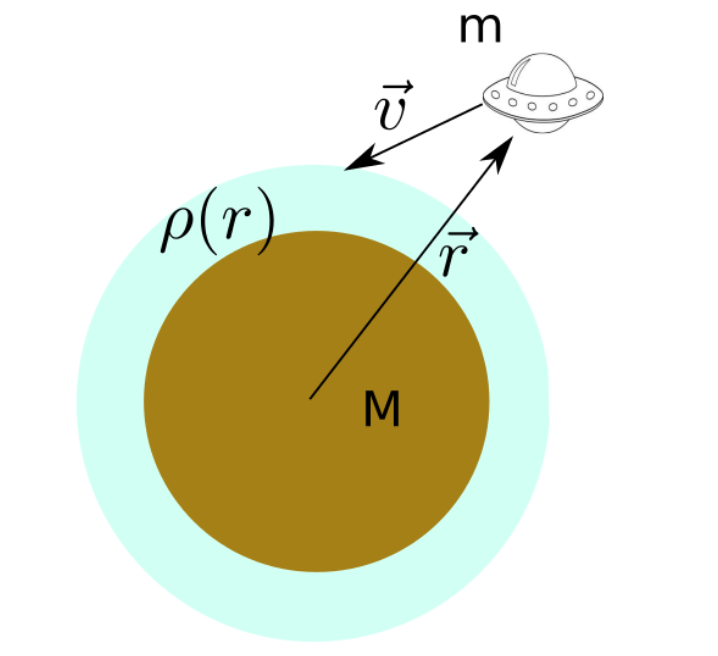
\includegraphics[scale=0.4]{media/landing.png}\\
{
\footnotesize
Velkommen til andre forelesning i del 1B! Under er det noen punkter til repetisjon.
Kun når du har \textcolor{red}{\bf full kontroll} på alt dette kan du gå videre. Hvis ikke, gå tilbake til forrige forelesning for å repetere litt eller spør foreleser og/eller gruppelærer hvis det er ting som er uklare. Dette forelesningsnotatet tilsvarer en og en halv fysisk dobbelttime, kanskje litt mindre.\\
{\bf Er du klar?}\ \ \ \ \ \hyperlink{conic1}{\pagebutton{Neste side}}
}
\column{0.5\textwidth}
{
\small
\begin{enumerate}
\item Kan du prøve å tenke gjennom hvordan du ville utledet tolegemeproblemet hvis du skal gjøre det igjen uten hjelp av forelesningsnotater? Du trenger ikke å gjøre alle stegene i detalj, men tenke gjennom, steg for steg, hva vi gjorde. Hvis du er usikker på noen av stegene kikk tilbake.
\item Klarer du å bruke Newtons lover på vektorform, inkludert derivasjoner og bruk av enhetsvektorer i polarkoordinater?
\item Kjenner du til alle begrepene og egenskapene til ellipser som du skal kjenne i kurset?
\end{enumerate}

}
%\movie[autostart]{testmovie}{launch.gif}%bate2.mpg
\end{columns}
\end{frame}


\begin{frame}
\label{conic1}
\lastpagebutton{intro}
Vi utledet at løsningen av tolegemeproblemet kan skrives som:
\[
r(f)=\frac{p}{1+e\cos{f}}
\]
der $p$ og $e$ er positive integrasjonskontstanter. Hvis $e<1$ så er dette formelen for en ellipse:
\[
r(f)=\frac{a(1-e^2)}{1+e\cos{f}}
\]
der det ene objektet er i brennpunktet:
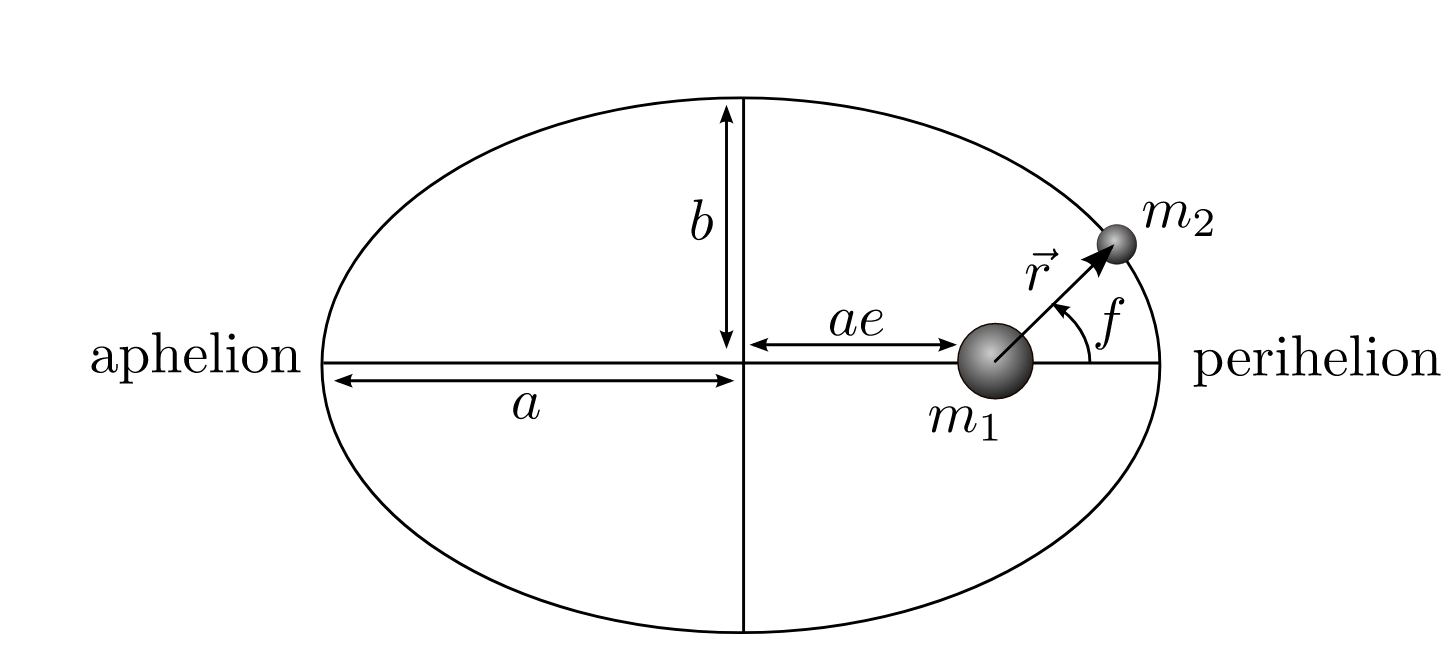
\includegraphics[scale=0.3]{media/ellipse.png}\hyperlink{feil_conic1b}{\pagebutton{Neste side}}
\end{frame}


{
\setbeamercolor{background canvas}{bg=black}
\begin{frame}
\label{feil_conic1b}
\lastpagebutton{conic1}
{\Huge
\textcolor{orange}{Men det store spørsmålet i forrige forelesning var:}\\
\textcolor{orange}{Hva hvis $e\ge1$????}\\
\textcolor{orange}{Da har vi ikke lenger en ellipsebane...}\\
\textcolor{orange}{Men hva har vi da...???}
}
\hyperlink{conic2}{\pagebutton{Neste side}}
\end{frame}
}




\begin{frame}
\label{conic2}
\lastpagebutton{feil_conic1b}
\addtocounter{pageno}{-1}
Likningen vi har kommet frem til er tilfeldigvis likningen for \textit{kjeglesnitt (conic sections)} i polarkoordinater. Vet du hvilke 3 typer kurver som inngår i kjeglesnittene? Den ene er ellipser ja, men de andre to?\\
\hyperlink{conic2_b}{\pagebutton{Trykk her når du har funnet ut av det}}\\
\textcolor{white}{Ganske riktig, {\it parabler} og {\it hyperbler}: }
\begin{columns}
\column{0.5\textwidth}
\centerline{\textcolor{white}{
  xxxx
  xxxx
  xxxx}
}
\column{0.5\textwidth}
\textcolor{white}{De sorte linjene er ellipser, den blå er en parabel mens den røde og grønne er hyperbler. Den sorte prikkete ellipsen har $e=0$ og er dermed en sirkel. Den heltrukne sorte linja er en ellipse med eksentrisitet $e=0.7$. Den sorte prikken er brennpunktet i sirkelen  (og dermed sentrum siden det er sirkel), den oransje prikken er brennpunktet i ellipsen.}
\textcolor{white}{Neste side}
\end{columns}
\end{frame}


\begin{frame}
\label{conic2_b}
\lastpagebutton{feil_conic1b}
\addtocounter{pageno}{-1}
Likningen vi har kommet frem til er tilfeldigvis likningen for \textit{kjeglesnitt (conic sections)} i polarkoordinater. Vet du hvilke 3 typer kurver som inngår i kjeglesnittene? Den ene er ellipser ja, men de andre to?\\
{\pagebutton{Trykk her når du har funnet ut av det}}\\
Ganske riktig, {\it parabler} og {\it hyperbler}:
\begin{columns}
  \column{0.5\textwidth}
\centerline{
  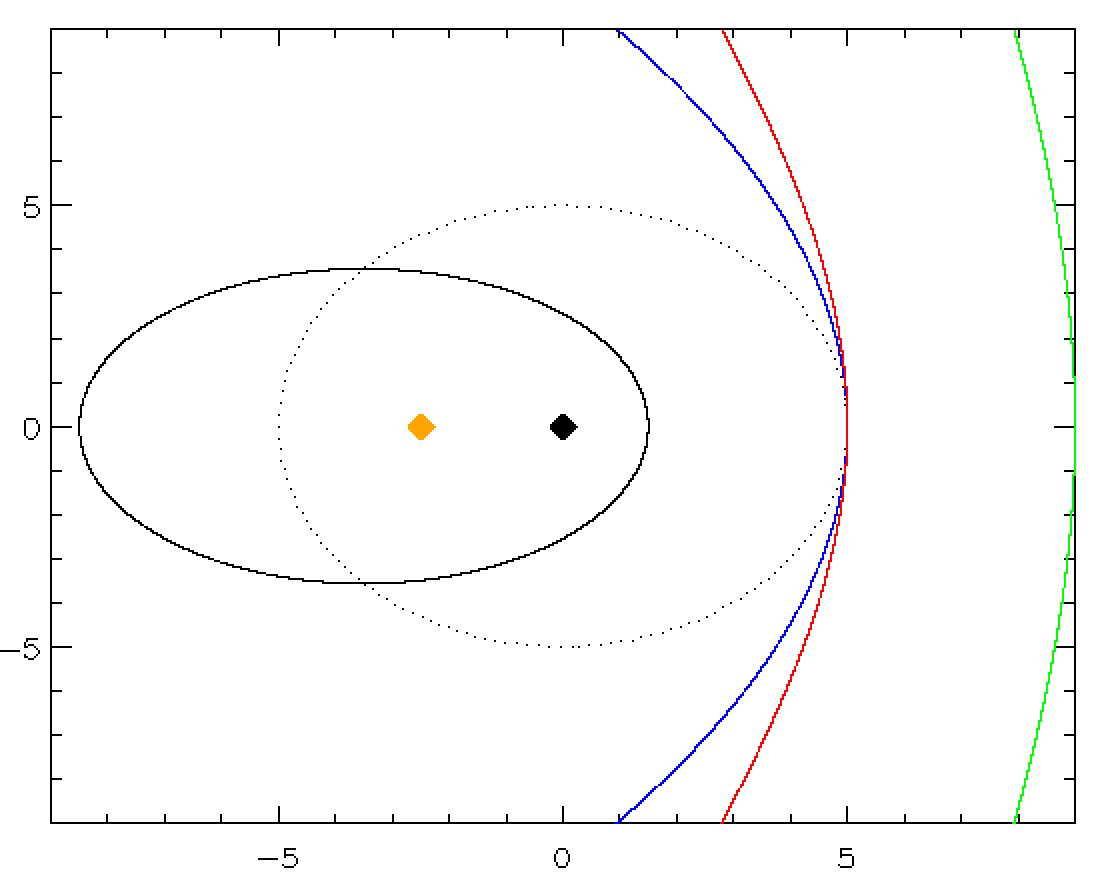
\includegraphics[height = 0.5\textheight, width = 0.75\textwidth]{media/conicsections0.png}
}
\column{0.5\textwidth}
De sorte linjene er ellipser, den blå er en parabel mens den røde og grønne er hyperbler. Den sorte prikkete ellipsen har $e=0$ og er dermed en sirkel. Den heltrukne sorte linja er en ellipse med eksentrisitet $e=0.7$. Den sorte prikken er brennpunktet i sirkelen  (og dermed sentrum siden det er sirkel), den oransje prikken er brennpunktet i ellipsen.
\hyperlink{blue_nytema1}{\pagebutton{Neste side}}
\end{columns}
\end{frame}







\renewcommand{\headline}{\small Kjeglesnitt}
{
\setbeamercolor{background canvas}{bg=blue}
\begin{frame}
\label{blue_nytema1}
\hyperlink{conic2}{\pagebutton{\small Forrige side}}
\nytemaside{euler4}
\textcolor{yellow}{La oss repetere litt om kjeglesnitt og se mer på uttrykket i polarkoordinater.}\\
\vspace*{0.5cm}
\hyperlink{conic3}{\pagebutton{Ja, hvordan var nå det igjen...}}
\end{frame}
}




\begin{frame}
\label{conic3}
\dlastpagebutton{blue_nytema1}
\begin{columns}
  \column{0.5\textwidth}
  \centerline{
  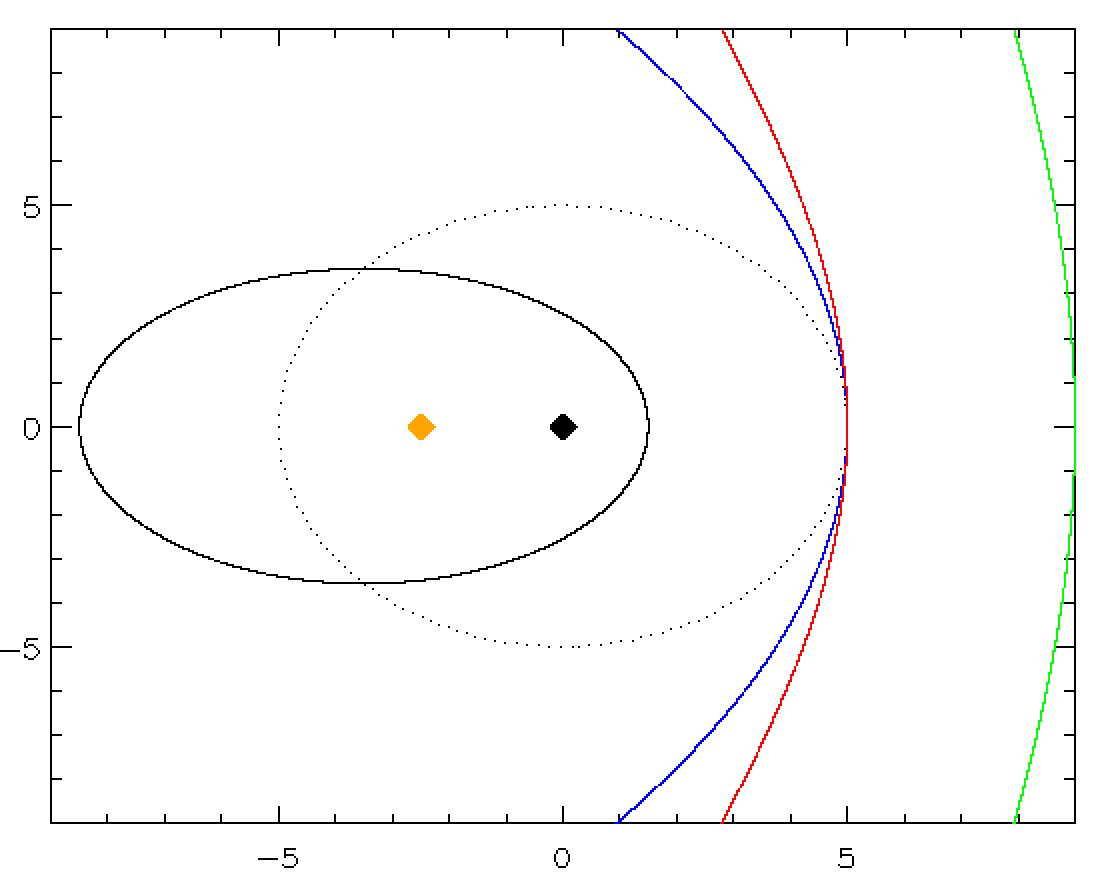
\includegraphics[height = 0.5\textheight, width = 0.75\textwidth]{media/conicsections0.png}
}
Hyperbler og parabler har også formel
\[
r(f)=\frac{p}{1+e\cos{f}}
\]
\column{0.5\textwidth}
men for
\begin{itemize}
\item parabler er $e=1$ og $p=2a$
\item hyperbler er $e>1$ og $p=-a(1-e^2)$
\item mens vi husker at ellipser hadde $e<1$ og $p=a(1-e^2)$
\end{itemize}
Merk at for ellipser og hyperbler så er det kun et minustegn som skiller uttrykket for $p$. Årsaken til minustegnet er for å holde $p$ positiv ($r$ må jo være en positiv størrelse) når $e$ plutselig har blitt større enn 1. I figuren til venstre så har alle kurvene $a=5$ mens de to hyperblene har $e=2$ (rød) og $e=2.8$ (grønn).
\hyperlink{feil_conic4}{\pagebutton{Neste side}}
\end{columns}
\end{frame}



{
\setbeamercolor{background canvas}{bg=black}
\begin{frame}
\label{feil_conic4}
\lastpagebutton{conic3}
{\huge
\textcolor{orange}{Så ja, Kepler fant faktisk ikke hele sannheten! Hvorfor ikke?\\
Fordi, som du ser fra figuren, objekter som går i parabelbaner og hyperbelbaner ikke er bundet til sola, de kommer bare innom men aldri tilbake igjen!\\
Slike objekter vil dermed ikke være fra vårt solsystem men være besøk fra det interstellar rom.
}}
\hyperlink{feil_conic5}{\pagebutton{Neste side}}
\end{frame}
}



{
\setbeamercolor{background canvas}{bg=black}
\begin{frame}
\label{feil_conic5}
\lastpagebutton{feil_conic4}
{\large
\textcolor{orange}{Det er først nå i det siste at man har oppdaget slike objekter. Det aller første ble oppdaget i 2017 og ble kalt {\it Oumuamua}. Her er en kunstrisk fremstilling av hvordan objektet kan se ut (credit: ESO/M. Kornmesser)\\
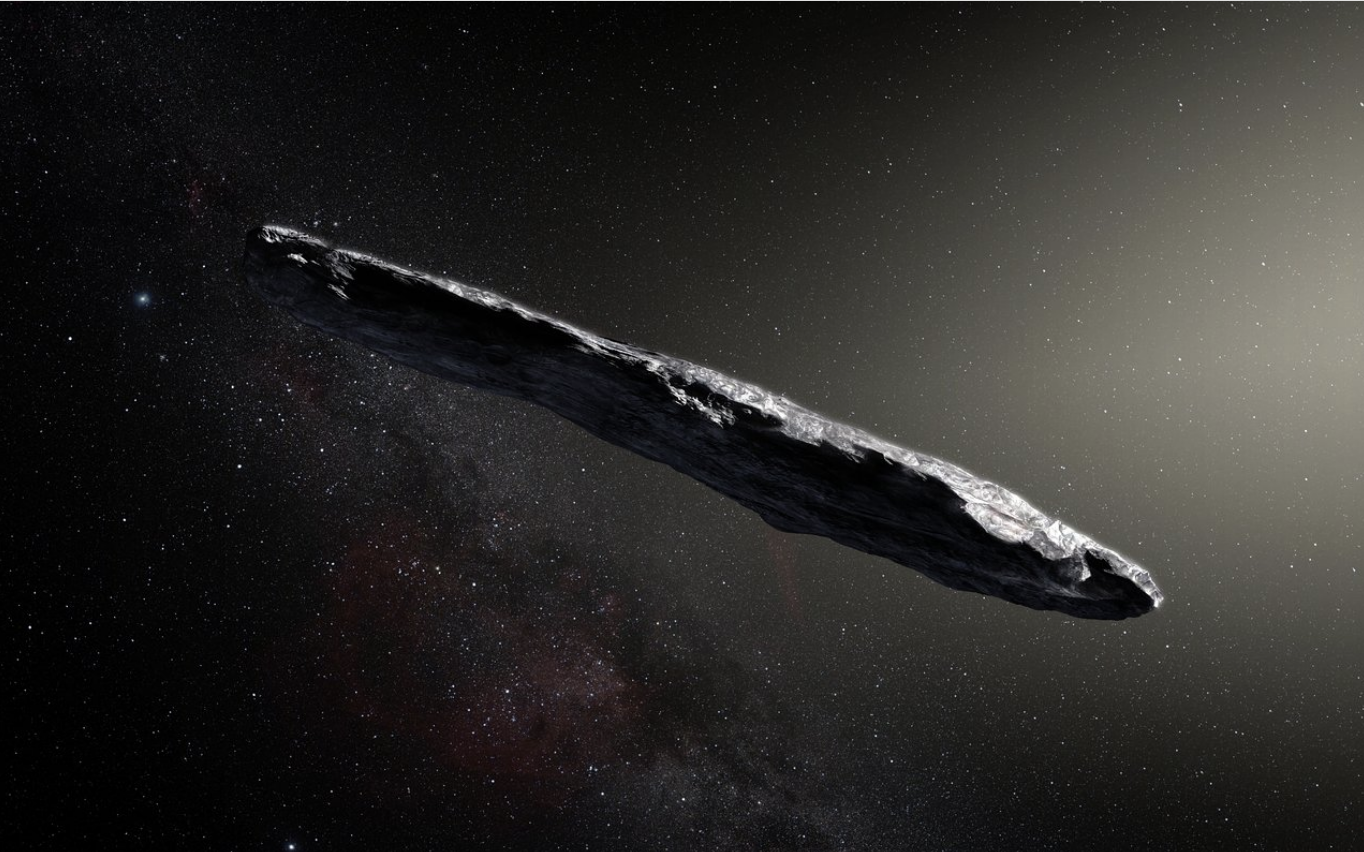
\includegraphics[scale=0.3]{media/oumuamua.png}
}}
\hyperlink{conic6}{\pagebutton{Neste side}}
\end{frame}
}


\begin{frame}
\label{conic6}
\lastpagebutton{feil_conic5}
Vi skal snart se litt på hva betingelsene er for at et objekt får en elliptisk, parabel eller hyperbelbane. Dette er jo spesielt viktig for satelitter. Hvis vi ønsker å ha en satelitt i bane rundt jorda så bør vi helst sørge for at den går i en ellipsebane. Ellers vil vi jo miste satelitten! Men før vi gjør det la oss kikke litt på ukeoppgavene.\\
Vi har her utledet Keplers 1.lov. Men hva med Keplers 2. og 3. lov? De skal du få lov til å utlede selv i oppgave 1B.1 og 1B.2.\\ 
\hyperlink{blue_nytema2}{\pagebutton{Neste side}}
\end{frame}

\renewcommand{\headline}{\small Keplers 2. og 3.lov}
{
\setbeamercolor{background canvas}{bg=blue}
\begin{frame}
\label{blue_nytema2}
\hyperlink{conic6}{\pagebutton{\small Forrige side}}
\nytemaside{xxx}
\textcolor{yellow}{Nå skal du få tyvtitte litt på oppgavene der du skal utlede Keplers 2. og 3. lov. Nå som vi har utledet Keplers første lov, så er det {\bf mye} enklere å utlede de to siste, lover!}\\
\vspace*{0.5cm}
\hyperlink{oppgaver1}{\pagebutton{Virkelig?}}
\end{frame}
}


\begin{frame}
\label{oppgaver1}
\begin{columns}
\column{0.4\textwidth}
\lastpagebutton{conic6}
\headlinebutton{\headline}\\
{\scriptsize
Tenk {\bf fort} gjennom hvordan du kan gå frem for å løse oppgave 1B.1 under her (prosjektstudenter har en liknende oppgave i utfording B1, del 2):
{\bf Deretter}, velg om du enten vil gå videre til neste side og heller se mer på oppgaven etter forelesningen {\bf eller} om du vil bruke litt tid på oppgaven nå. Hvis du vil se litt mer på oppgaven nå: tenk litt til og hvis du sitter helt fast, ta gjerne en titt på \href{https://www.uio.no/studier/emner/matnat/astro/AST2000/h20/undervisningsressurser/interaktive-forelesningsnotater/1b/videoer/video1b_9.mp4}{denne videoen} for noen tips. \textcolor{red}{Merk at det ikke er meningen at du skal løse oppgaven nå men finne din egen ide om hvordan du ville startet på hver av deloppgavene. Ikke se på videoen før du har egne forslag.}}
\column{0.5\textwidth}
\hspace*{-0.5cm}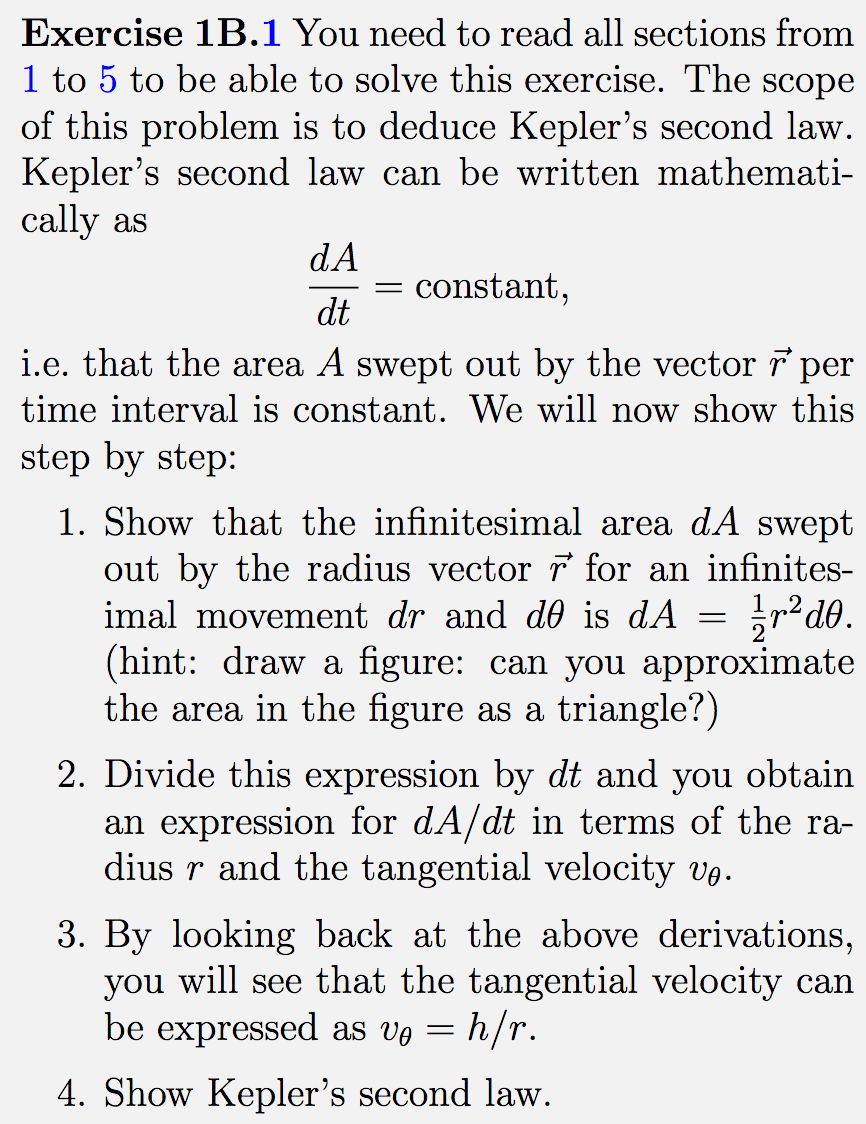
\includegraphics[scale=0.43]{media/1b1.png}
\hyperlink{oppgaver2}{\pagebutton{Neste side}}
\end{columns}
\end{frame}


\begin{frame}
\label{oppgaver2}
\begin{columns}
\column{0.4\textwidth}
\lastpagebutton{oppgaver1}
\headlinebutton{\headline}\\
Tenk  {\bf fort} gjennom hvordan du kan gå frem for å løse deloppgave 1 og 3 fra oppgave 1B.2 under her (prosjektstudenter har en liknende oppgave i utfording B1, del 2): Etter at du har tenkt, ta gjerne en titt på \href{https://www.uio.no/studier/emner/matnat/astro/AST2000/h20/undervisningsressurser/interaktive-forelesningsnotater/1b/videoer/video1b_10.mp4}{denne videoen} for noen tips.\textcolor{red}{ Merk at det ikke er meningen at du skal løse oppgaven nå men finne din egen ide om hvordan du ville startet på hver av deloppgavene. Ikke se på videoen før du har egne forslag.}
\column{0.45\textwidth}
\hspace*{-0.5cm}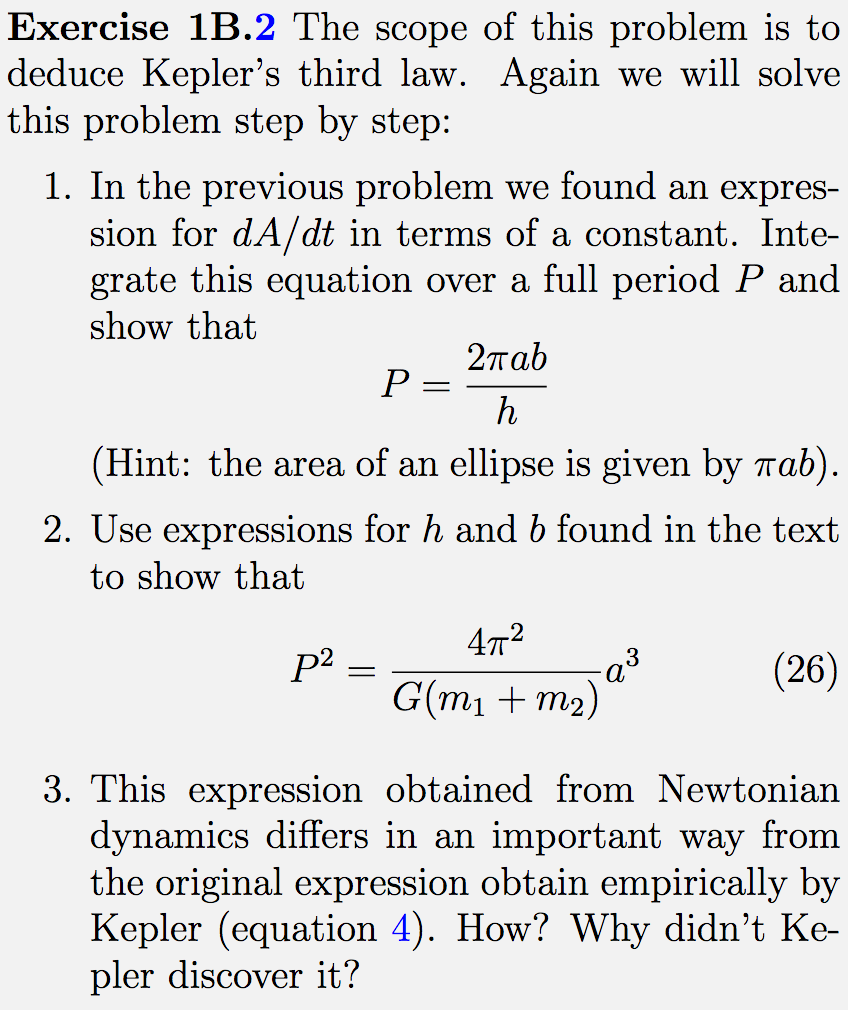
\includegraphics[scale=0.43]{media/1b2.png}
\hyperlink{oppgaver3}{\pagebutton{Neste side}}
\end{columns}
\end{frame}


\begin{frame}
\label{oppgaver3}
\lastpagebutton{oppgaver2}
Spesielt den siste oppgaven her er {\bf svært} viktig!
\begin{alertblock}{\bf Keplers 3.lov}
Du utledet i oppgaven at Keplers versjon av sin 3.lov er noe gal. Det er svært viktig å bruke den riktige formelen i alt som vi gjør i dette kurset her. Den riktige formelen (som også er i SI-enheter) er gitt ved
\[
P^2=\frac{4\pi^2}{G(m_1+m_2)}a^3
\]
Vi ser at begge massene er med på å bestemme forholdet mellom omløpsperiode og store halvakse i en ellipsebane!
\end{alertblock}
\hyperlink{oppgaver4}{\pagebutton{Neste side}}
\end{frame}

\begin{frame}
\label{oppgaver4}
\lastpagebutton{oppgaver3}
Før vi går videre, ta en nøye titt på første deloppgave av oppgave 1B.3:\\
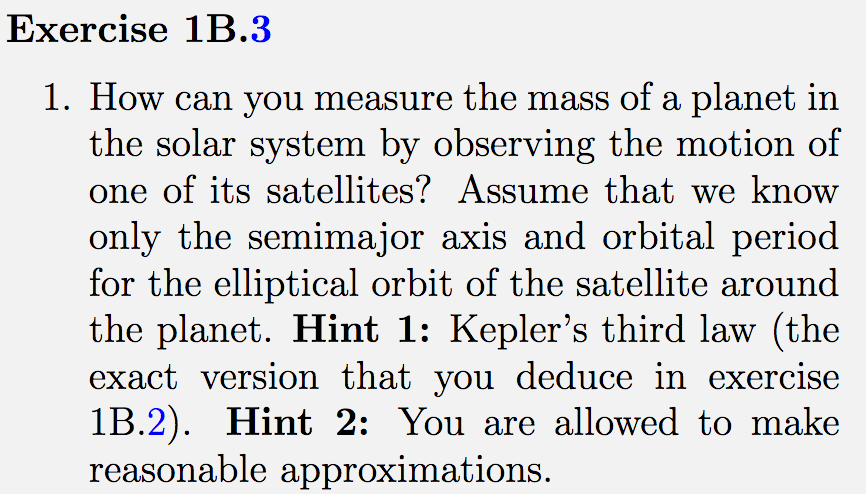
\includegraphics[scale=0.4]{media/1b3.png}\\
Tenk i maks 2-3 minutter om du ser en måte å løse den på? Hvis ikke, ta det etter forelesningen.
\hyperlink{cm1}{\pagebutton{Neste side}}
\end{frame}

\renewcommand{\headline}{\small 2-legemeproblemet igjen}

\begin{frame}
\label{cm1}
\lastpagebutton{oppgaver4}
Men stopp en hal! Har vi egentlig løst 2-legemeproblemet? Vi har løst problemet i tilfellet hvor vi setter oss på $m_1$ og ser på bevegelsen til $m_2$ som da blir en ellipsebane med $m_1$ i det ene brennpunktet. Men hva hvis vi setter oss på $m_2$? Likningene vi får blir jo de samme, så løsningen blir den samme med massene byttet om, $m_2$ står i et brennpunkt til ellipsebanen som $m_1$ følger. Men hva hvis vi nå befinner oss et punkt langt vekk og ser legemene på avstand mens vi ikke befinner oss i referansesystemet til noen av dem? Hvordan vil da $m_1$ og $m_2$ bevege seg?\\
Tenk deg godt om før du går til neste side...
\hyperlink{blue_nytema3}{\pagebutton{Neste side}}
\end{frame}

\renewcommand{\headline}{\small Massesenter}
{
\setbeamercolor{background canvas}{bg=blue}
\begin{frame}
\label{blue_nytema3}
\hyperlink{cm1}{\pagebutton{\small Forrige side}}
\nytemaside{xxx}
\textcolor{yellow}{Vi skal repetere noe du kjenner godt, og bruke dette til å gjøre det fulle 2-legeme-problemet litt enklere å løse.}\\
\vspace*{0.5cm}
\hyperlink{cm2}{\pagebutton{Massesenter, kan godt trenge en kjapp repetisjon ja...}}
\end{frame}
}


\begin{frame}
\label{cm2}
\lastpagebutton{cm1}
{\small For å finne svaret, må vi repetere et uttrykk som du allerede kjenner: {\it massesenter.}}\\
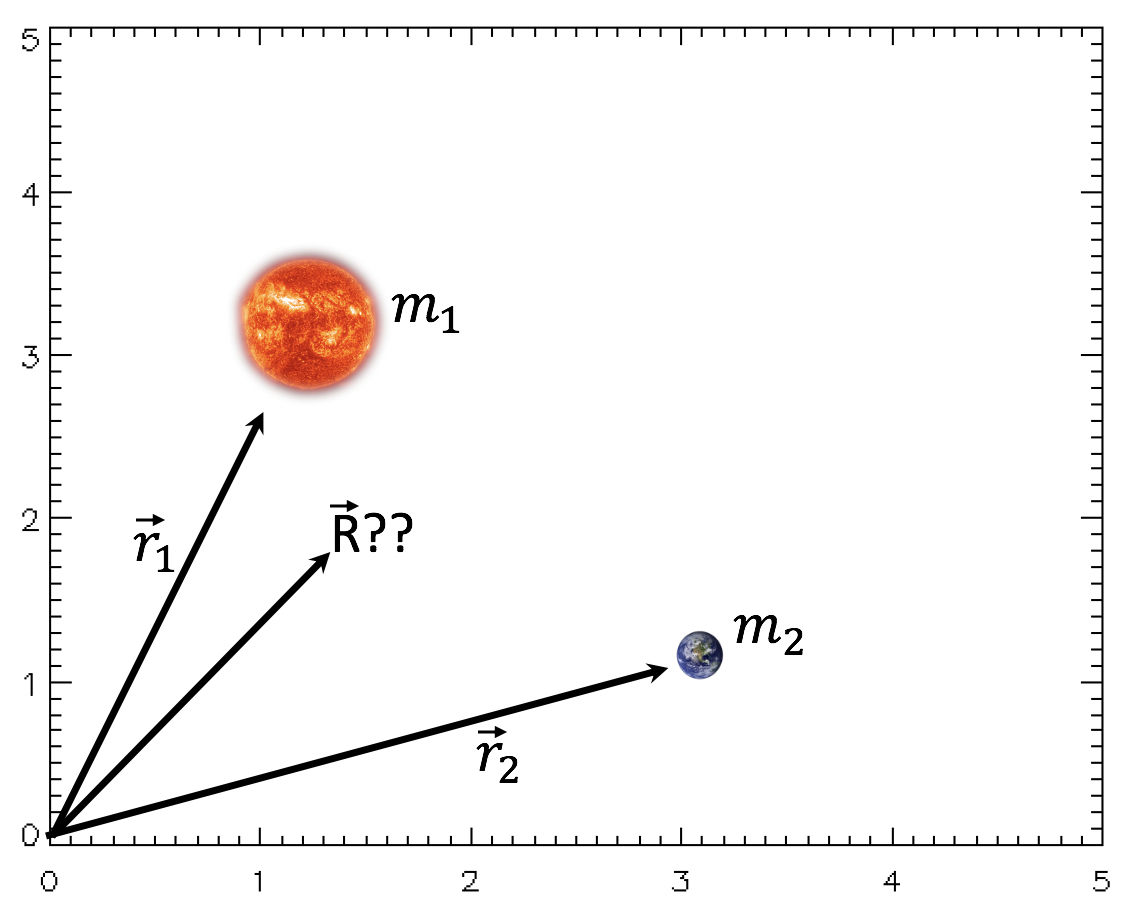
\includegraphics[scale=0.35]{media/cm1.png}\\
Hvis vi kjenner posisjonene $\vec{r_1}$ og $\vec{r_2}$ på figuren, hvordan kan vi da finne posisjonen $\vec{R}$ til massesenteret? Du kan bruke massene $m_1$ og $m_2$. Hva er formelen?\\
\hyperlink{cm3}{\pagebutton{Trykk her når du har frisket opp massesenterdefinisjonen!}}
\end{frame}


\begin{frame}
\label{cm3}
\lastpagebutton{cm2}
\addtocounter{pageno}{-1}
Stemmer! Vi må rett og slett ta midlet mellom de to posisjonene, vektet med massene:
\[
\vec{R}=\frac{m_1\vec{r_1}+m_2\vec{r_2}}{m_1+m_2}
\]
Men hva hvis vi nå skal finne massesenteret $\vec{R}$ til en galakse og vi kjenner posisjonene $\vec{r_i}$ til alle $N$ stjernene med masse $m_i$ i galaksen? (anta at det ikke finnes annen masse i galaksen). Hvordan kan vi generalisere uttrykket vårt??\\
\hyperlink{cm3_b}{\pagebutton{Diskuter og trykk her når du har funnet ut av det}}\\
\textcolor{white}{
Vi bare midler på samme måte over alle objekter:
\[
\vec{R}=\frac{1}{M}\sum_{i=1}^Nm_i\vec{r_i}
\]
Her er $M$ summen over alle massene. Pass på at du har denne friskt i minne videre...
{Neste side}}
\end{frame}

\begin{frame}
\label{cm3_b}
\lastpagebutton{cm2}
\addtocounter{pageno}{-1}
Stemmer! Vi må rett og slett ta midlet mellom de to posisjonene, vektet med massene:
\[
\vec{R}=\frac{m_1\vec{r_1}+m_2\vec{r_2}}{m_1+m_2}
\]
Men hva hvis vi nå skal finne massesenteret $\vec{R}$ til en galakse og vi kjenner posisjonene $\vec{r_i}$ til alle $N$ stjernene med masse $m_i$ i galaksen? (anta at det ikke finnes annen masse i galaksen). Hvordan kan vi generalisere uttrykket vårt??\\
\hyperlink{cm3a}{\pagebutton{Diskuter og trykk her når du har funnet ut av det}}\\
Vi bare midler på samme måte over alle objekter:
\[
\vec{R}=\frac{1}{M}\sum_{i=1}^Nm_i\vec{r_i}
\]
Her er $M$ summen over alle massene. Pass på at du har denne friskt i minne videre...
\hyperlink{cm4}{\pagebutton{Neste side}}
\end{frame}







\begin{frame}
\label{cm4}
\dlastpagebutton{cm3}
For å kunne finne bevegelsen til både $m_1$ og $m_2$ skal vi nå utlede en utvidelse av Newtons 2.lov som gjelder for et mangelegemesystem. Anta igjen at vi har galaksen vår med N stjerner og at det mellom disse kun virker gravitasjonskrefter $\vec{f_{ij}}$ (krafta på legeme $i$ fra legeme $j$). I tillegg kan det virke en ekstern kraft $\vec{F}_\mathrm{ext}$ som virker likt på hele systemet, dvs. på alle objektene, f.eks. en annen galakse som trekker på galaksen. I \href{https://www.uio.no/studier/emner/matnat/astro/AST2000/h20/undervisningsressurser/interaktive-forelesningsnotater/1b/videoer/video1b_11.mp4}{denne videoen} blir du satt igang med utledningen av Newtons 2.lov på mangelegemesystemer.\\
Etter å ha sett videoen skal du nå se om du kan komme frem til et uttrykk av typen:
\[
\vec{F}=\Sigma\Sigma \vec{f}+\vec{F}_\mathrm{ext}=\Sigma m\vec{r}
\]
og sett inn riktige indekser på krefter, masser, posisjonsvektorer og tidsderiverte. Pass spesielt på at summegrensene blir riktige! Bruk maks 5 minutter.
\hyperlink{cm5}{\pagebutton{Neste side}}
\end{frame}

\begin{frame}
\label{cm5}
\lastpagebutton{cm4}
{\bf Vi skal nå forenkle dette uttrykket:}
Ved å bruke 
\begin{itemize}
\item en av Newtons lover som sier noe om krefter som er lik hverandre, dette skal gi deg at et av leddene er 0
\item massesenterdefinisjonen $\vec{R}=\frac{1}{M}\sum_{i=1}^Nm_i\vec{r_i}$
\end{itemize}
skal du vise at
\[
\vec{F}_\mathrm{ext}=M\ddot{\vec{R}}
\]
som er Newtons 2.lov for mangelegemesystemer. Fikk du det til?\\
Hvis du er usikker, se på \href{https://www.uio.no/studier/emner/matnat/astro/AST2000/h20/undervisningsressurser/interaktive-forelesningsnotater/1b/videoer/video1b_12.mp4}{denne videoen}.\\
Før du går til neste side, prøv å si til hverandre med ord hva denne likningen sier. Ser du hva essensen er?
\hyperlink{cm6}{\pagebutton{Neste side}}
\end{frame}


\renewcommand{\headline}{\small 2-legemeproblem sett fra massesenter}

\begin{frame}
\label{cm6}
\lastpagebutton{cm5}
Hva hvis de eksterne kreftene på systemet er null?\\
Da er $\ddot{\vec{R}}=0$ og massesenteret har ingen akselerasjon! Massesenteret vil da kun bevege seg med konstant hastighet. Vi kan da dele bevegelsen til en stjerne i galaksen opp i 
\begin{itemize}
\item bevegelsen til stjerna i forhold til massesenteret PLUSS
\item bevegelsen til massesenteret
\end{itemize}
Hvis det ikke er noen ytre krefter så vil massesenterbevegelsen være enkel, konstant hastighet. Da trenger vi kun å finne bevegelsen til stjerna om massesenteret.\\
\textcolor{red}{Dette hjelper oss med tolegemeproblemet vårt: vi trenger dermed kun å finne bevegelsen til de to legemene omkring deres felles massesenter.}
\hyperlink{pause}{\pagebutton{Neste side}}
\end{frame}

{
\setbeamercolor{background canvas}{bg=cyan}
\begin{frame}
\label{pause}
\hyperlink{cm6}{\pagebutton{\small Forrige side}}
{\Huge
\centerline{TID FOR KAFFEPAUSE!!!}
\centerline{
\includegraphics[scale=4]{media/drink-coffee.png}}\\

Ut å strekke på bena. Inn med litt koffein...\\
\vspace*{0.5cm}
Ihvertfall 10 min...
}\\
\vspace*{0.5cm}
{\tiny I den fysiske forelesningen kommer vi noen få sider til før den andre dobbelttimen er over. Hvis du følger anbefalingene mine og idag begynte der du slapp på forrige forelesningsnotat, så tar du noen få sider til og gir deg for idag. Etter det skal det stå igjen ca. en halv dobbelttime fysisk forelesning.}
\vspace*{0.5cm}
\hyperlink{cm7}{\pagebutton{Jeg lover, jeg har tatt pause og er klart til å fortsette}}
\end{frame}
}

\begin{frame}
\label{cm7}
\begin{columns}
\column{0.5\textwidth}
\lastpagebutton{cm6}
Her har vi situasjonen:\\
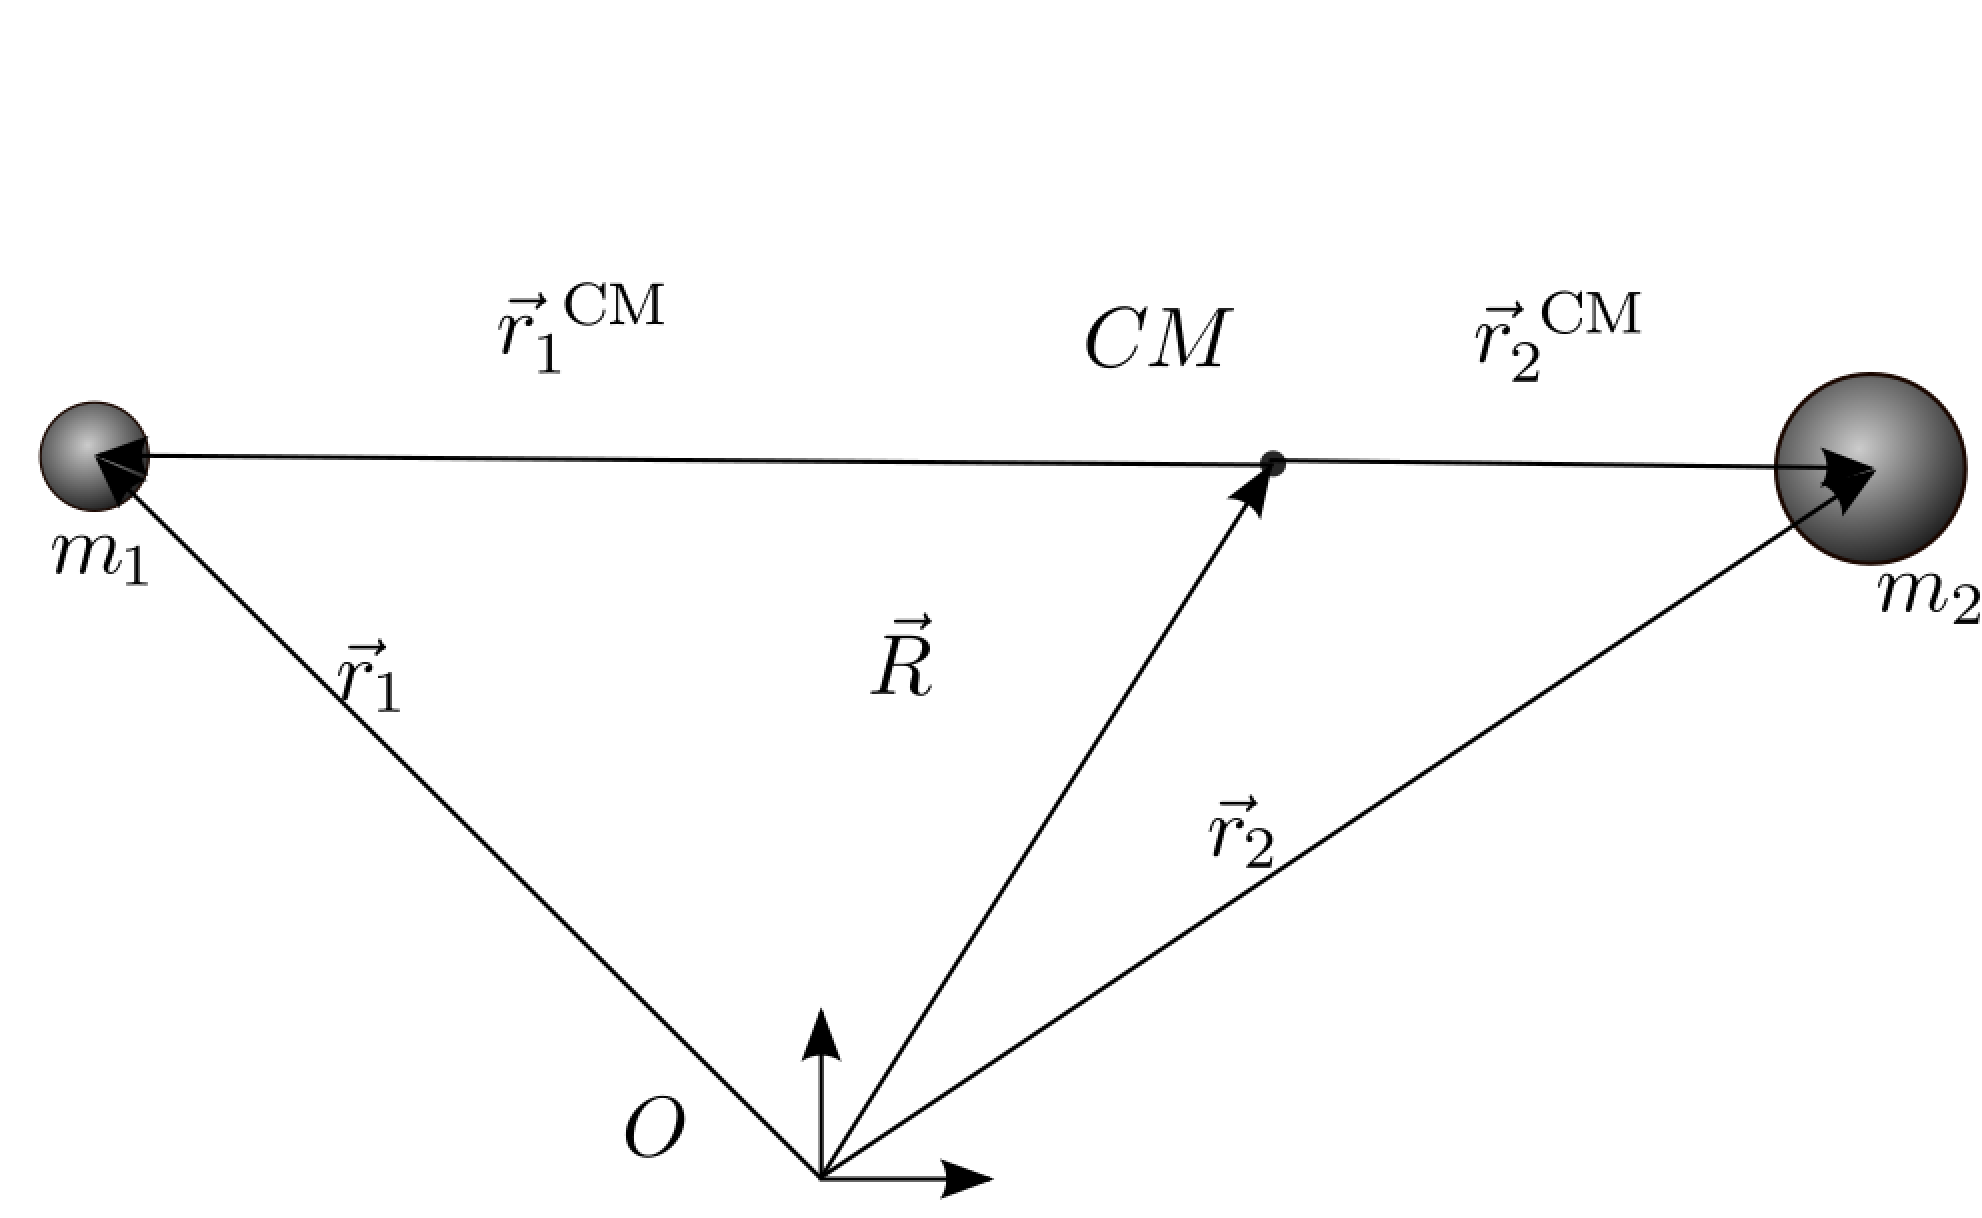
\includegraphics[scale=0.17]{media/cm3.png}\\
Fra et gitt origo O utenfor systemet så har vi poisjonsvektorene $\vec{r_1}$ og $\vec{r_2}$ som peker på de to legemene, samt $\vec{R}$ som peker på massesenteret (CM, Center of Mass) til de to legemene. Vi er interessert i disse legemenes bevegelse i forhold til massesenteret (se forrige side hvis du er usikker på hvorfor!). 
\column{0.5\textwidth}
Da velger vi å flytte origo til massesenteret. Dette nye koordinatsystemet kaller vi massesentersystemet. Posisjonsvektorene $\vec{r_1}^{CM}$ og $\vec{r_2}^{CM}$ fra det nye origo er tegnet inn i figuren. Men hva med $\vec{R}^{CM}$. Hva er posisjonsvektoren til massesenteret fra dette nye origo?\\
Diskuter og tenk deg nøye om (1-2 min) før du ser på svaret på neste side. Svaret er kanskje enklere enn du tror...
\hyperlink{cm8}{\pagebutton{Neste side}}
\end{columns}
\end{frame}

\begin{frame}
\label{cm8}
\lastpagebutton{cm7}
\small
Siden poisjonen til massesenteret i massesenteret er i origo selv: $\vec{R}^{CM}=0$!\\
Nå til litt regning. Finn frem papir og blyant og forbered deg på å leke litt med likninger (ikke mye, gjør du det riktig så er dette fort gjort). 
\begin{block}{\bf Legemenes bevegelse om massesenteret}
{\small
Bruk nå massesentersystemet (sjekk forrige side hvis du har glemt ...), og {\bf sett inn i definisjonen av massesenteret for $\vec{R}$}. Gjør følgende substitusjoner:
\[
\vec{r} = \vec{r_2} - \vec{r_1}\ \ \ \mathrm{og}\ \ \ \hat\mu = \frac{m_1m_2}{m_1+m_2}
\]
MERK at vi har fjernet CM fra symbolene, i fortsettelsen så betyr $\vec{r}_1$ og $\vec{r}_2$ egentlig alltid $\vec{r}_1^{CM}$ og $\vec{r}_2^{CM}$! Den første liknigen her har vi brukt helt fra starten av: $\vec{r}$ var vektoren som pekte fra $m_1$ til $m_2$. Den andre er definisjonen av {\it redusert masse}. Den er mest for å gjøre likningene pene, men vi skal snart se at det også har en tolkning. Fra dette skal du komme frem til et uttrykk for $\vec{r_1}$.Altså: (1) du skal ta utgangspunkt i definisjon av massesenteret som nå er i origo, og (2) deretter bli kvitt $\vec{r_2}$ ved hjelp av uttrykket over og få inn $\mu$. Hva får du?
}
\end{block}
\hyperlink{feilr1}{\choicebutton{\small $\vec{r_1}=\hat\mu\vec{r}$}}\ \ \ \ \ \hyperlink{feilr1}{\choicebutton{\small $\vec{r_1}=\frac{m_1}{\hat\mu}\vec{r}$}}\ \ \ \ \ \hyperlink{feilr1}{\choicebutton{\small $\vec{r_1}=\frac{m_1}{\hat\mu}$}}\ \ \ \ \ \hyperlink{feilr1}{\choicebutton{\small $\vec{r_1}=-\frac{m_2}{\hat\mu}\vec{r}$}}\ \ \ \ \ \hyperlink{riktigr1}{\choicebutton{\small $\vec{r_1}=-\frac{\hat\mu}{m_1}\vec{r}$}}\ \ \ \ \ \hyperlink{feilr1}{\choicebutton{\small $\vec{r_1}=-\frac{\hat\mu}{m_2}\vec{r}$}}\ \ \ \ \ \hyperlink{feilr1}{\choicebutton{\small $\vec{r_1}=\frac{m_1}{m_2}\hat\mu\vec{r}$}}
\end{frame}


{
\setbeamercolor{background canvas}{bg=black}
\begin{frame}
\label{feilr1}
\lastpagebutton{cm8}
\textcolor{white}{Det ble galt! Prøv igjen. Husk at $\vec{R}=0$ i massesentersystemet. Og du kan bli kvitt $\vec{r_2}$ med uttrykket for $\vec{r}$. Da står du igjen med en likning med kun $\vec{r_1}$ og $\vec{r}$ som du løser for $\vec{r_1}$. Og til slutt erstatter du $m_1$ eller $m_2$ med $\hat\mu$, du vil nå ganske greit se hvordan $\hat\mu$ kommer inn her.\\
Hjelper det deg? Prøv igjen med dette som utgangspunkt!\\
(HUSK at vi nå har fjernet CM fra alle symbolene for å gjøre skrivingen lettere, alle vektorer har nå origo i massesenteret.)
}
\end{frame}
}

{
\setbeamercolor{background canvas}{bg=yellow}
\begin{frame}
\label{riktigr1}
\clastpagebutton{cm8}
{\bf STEMMER!} Nå som du har funnet $\vec{r_1}$, så kan du se om du klarer å vise at
\[
\vec{r_2}=\frac{\hat\mu}{m_2}\vec{r}
\]
Vi har dermed banene til de to legemene om massesenteret:
\begin{align}
\vec{r_1}&=-\frac{\hat\mu}{m_1}\vec{r}\\
\vec{r_2}&=\frac{\hat\mu}{m_2}\vec{r}
\end{align}
Men vi ser enda ikke hva slags form banen har. La oss ta absoluttverdiene til disse likningene. Bruk deretter det du vet om $r=|\vec{r}|$ (Jepp, dette er den samme som vi utledet i forrige forelesning, det er jo avstanden mellom de to objektene). Ser du nå hva slags baner de to legemene får om massesenteret (anta at det er bundet)?
\hyperlink{riktig_ja}{\choicebutton{JA, kult, nå ser jeg det!}}\ \ \ \ \ \hyperlink{feil_nei}{\choicebutton{Kanskje det, men jeg er litt usikker}}
\end{frame}
}

{
\setbeamercolor{background canvas}{bg=black}
\begin{frame}
\label{feil_nei}
\lastpagebutton{riktigr1}
\textcolor{white}{La oss først se hvordan likningene blir hvis vi tar absoluttverdi:
\begin{align}
|\vec{r_1}|&=r_1=\frac{\hat\mu}{m_1}|\vec{r}|=\frac{\hat\mu}{m_1}r\\
|\vec{r_2}|&=r_2=\frac{\hat\mu}{m_2}|\vec{r}|=\frac{\hat\mu}{m_2}r
\end{align}
Her er $r_1$ og $r_2$ avstanden til de to legemene fra massesenteret, ser du det? Disse avhenger jo av en vinkel $f$ ettersom de går i bane rundt massesenteret. I tillegg så fant vi jo i forrige forelesning et uttrykk for $r$ som inneholder en vinkel $f$. Da skulle du få uttrykk for $r_1$ og $r_2$ som inneholder vinklen $f$. Hjelper det deg?
\hyperlink{riktig_ja}{\pagebutton{Neste side}}
}
\end{frame}
}

{
\setbeamercolor{background canvas}{bg=yellow}
\begin{frame}
\label{riktig_ja}
\clastpagebutton{riktigr1}
{\small Fant du det? Innser du at begge legemene går i ellipser omkring massesenteret?}\\
\begin{columns}
\column{0.5\textwidth}
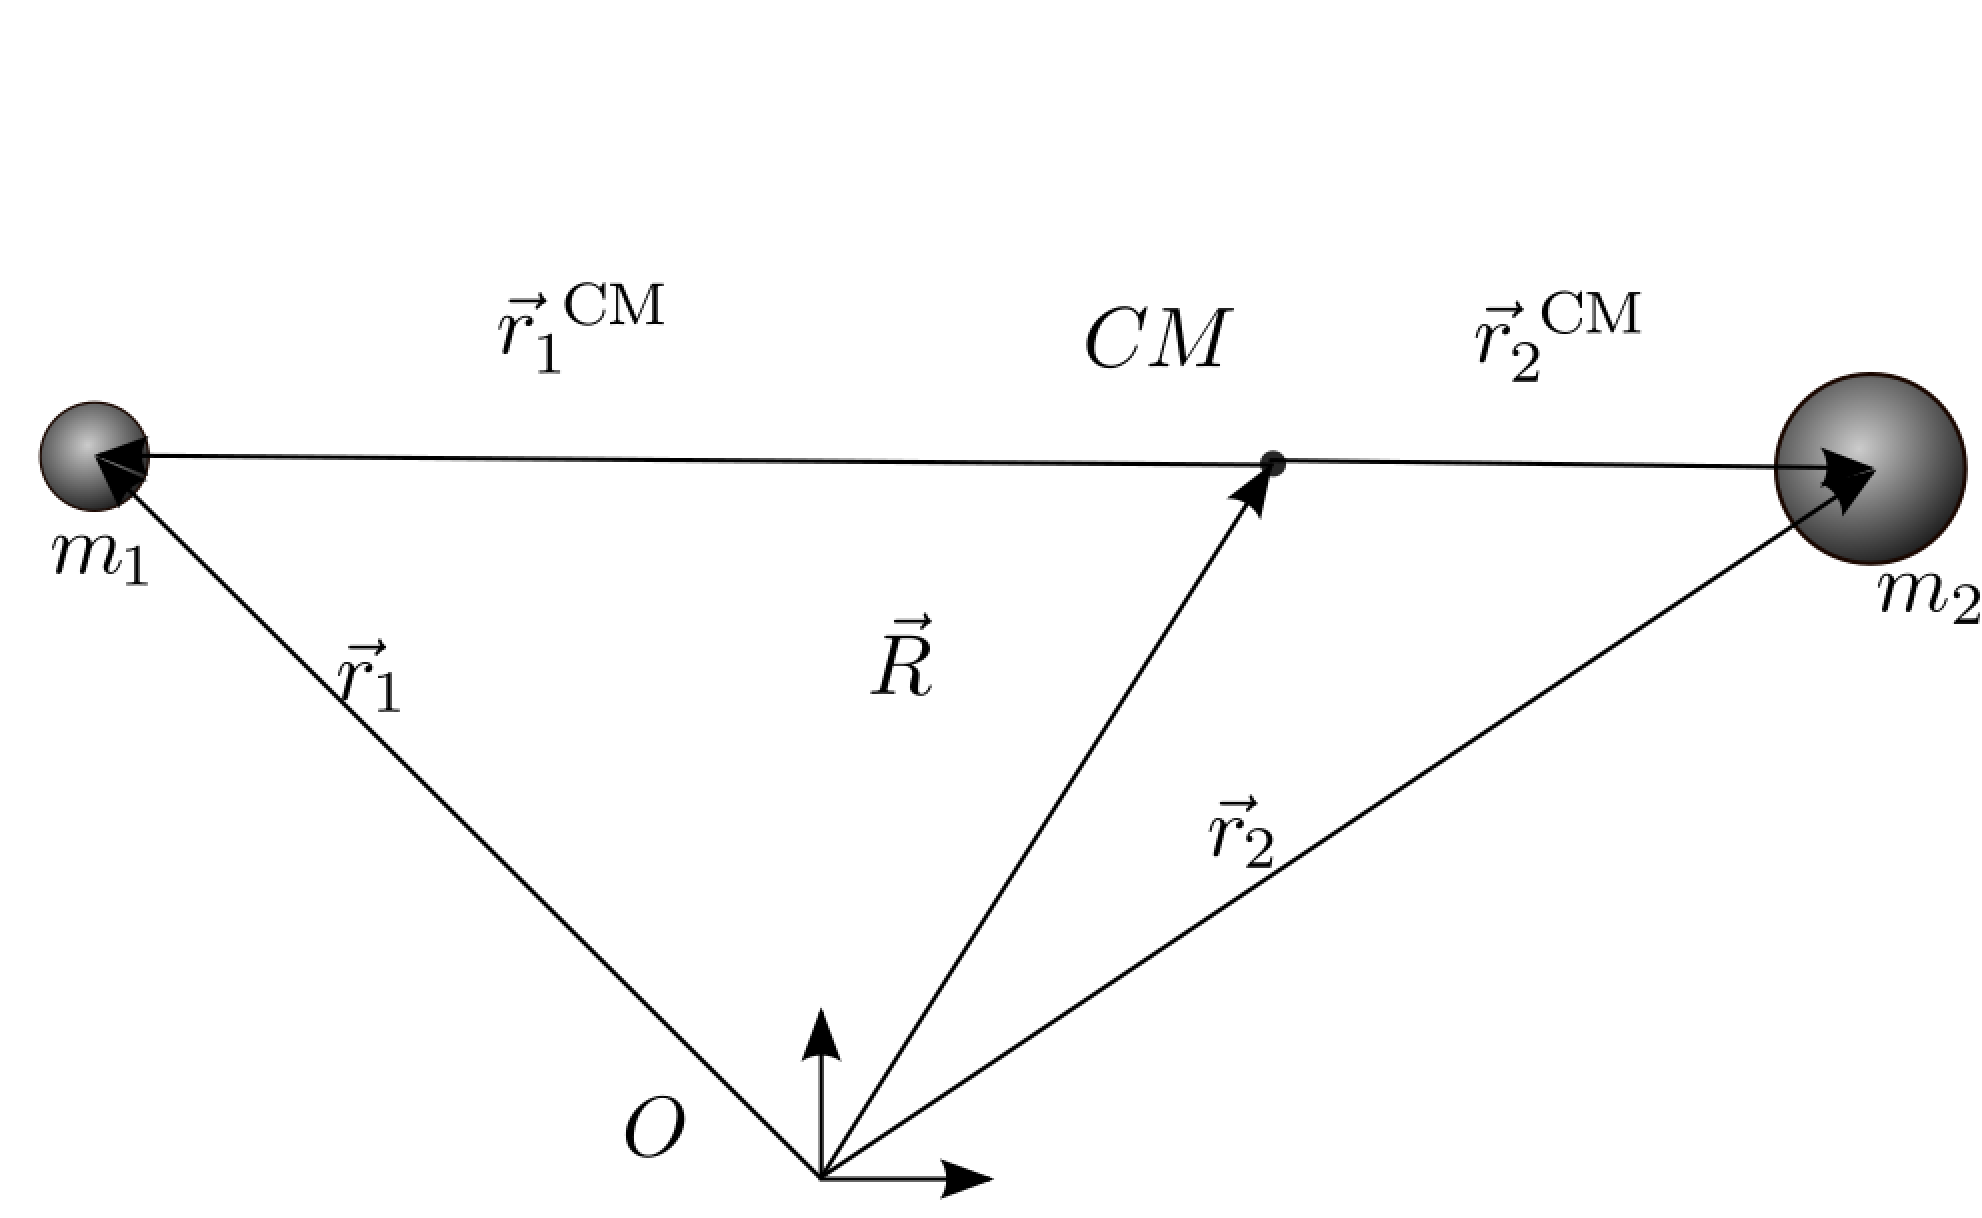
\includegraphics[scale=0.17]{media/cm3.png}
\column{0.5\textwidth}
\begin{align}
\vec{r_1}&=-\frac{\hat\mu}{m_1}\vec{r}\\
\vec{r_2}&=\frac{\hat\mu}{m_2}\vec{r}
\end{align}
\end{columns}
{\bf (MINNER IGJEN OM at vi nå har fjernet CM fra alle symbolene for å gjøre skrivingen lettere, alle vektorer har nå origo i massesenteret slik at $\vec{r_1}$ og $\vec{r_2}$ tilsvarer $\vec{r_1}^{CM}$ og $\vec{r_2}^{CM}$ på figuren.)}
{\small Ser du at ved å ta absoluttverdien på begge sider her, så har du likningene for $r_1(f)$ og $r_2(f)$ som altså er lengdene av vektorene $\vec{r_1}$ og $\vec{r_2}$. Disse viser altså banene til $m_1$ og $m_2$ som funksjon av en gitt vinkel $f$. Mens $r$ (eller egentlig $r(f)$) som står på høyre side i likningen er lengden $\vec{r}$ som vi utledet i forrige forelesning, altså banen til $m_2$ omkring $m_1$. Hvis denne er en ellipsebane ser du da at også $r_1(f)$ og $r_2(f)$ blir likninger for ellipser med massesenteret som brennpunkt?\\
}
\hyperlink{ja2}{\pagebutton{Neste side}}
\end{frame}
}


\begin{frame}
\label{ja2}
\lastpagebutton{riktig_ja}
Hva er de store halvaksene $a_1$ og $a_2$ til disse to ellipsene? Og hva er eksentrisiteten $e$?? Uttrykk svaret ved hjelp av massene og egenskapene til ellipsen som vi så på tidligere: nemlig ellipsebanen som det ene objektet har rundt det andre. Ved å sammenlikne uttrykkene for $r_1$ og $r_2$ som funksjon av $f$ som du nå har funnet, og sammenlikner med formelen for ellipse, så bør dette falle rett ut.\\
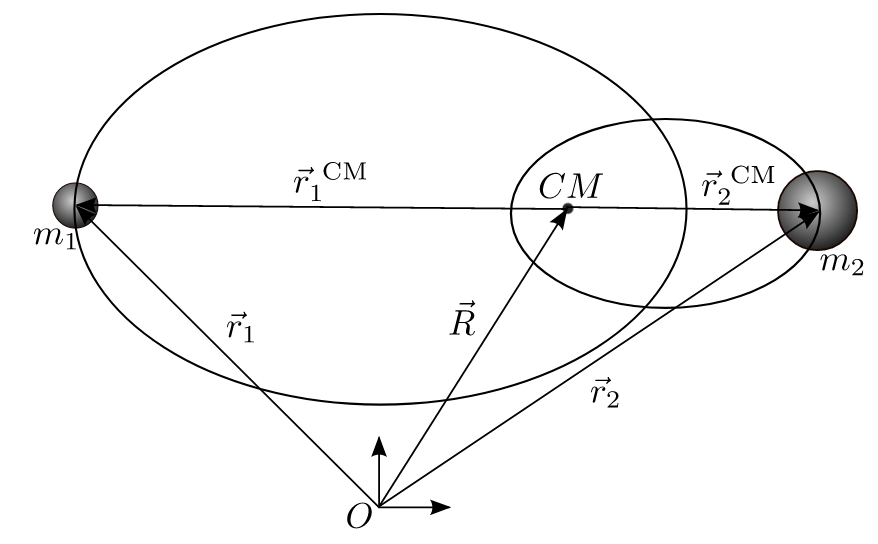
\includegraphics[scale=0.4]{media/cm2.png}\\
\hyperlink{cm9}{\pagebutton{Jeg har tenkt og tror jeg har svaret}}\\
Hvis du ikke har svaret, må du spørre foreleser/gruppelærer før du går videre. Det er veldig viktig at du har dette klart for deg nå!
\end{frame}



\begin{frame}
\label{cm9}
\lastpagebutton{ja2}
{\small
La oss først klare opp i begreper her, viktig at du har oversikt:
\begin{itemize}
\item Vektoren $\vec{r}$ peker fra det ene legemet til det andre. Lengden $r(f)$ av denne vektoren som avhenger av vinkelen $f$ som definert tidligere utgjør ellipsebanen til det ene legemet omkring det andre. Denne ellipsebanen har store halvakse lik $a$ og eksentrisitet $e$. {\bf Merk at sett fra referansesystemet til et av legemene (systemet der det ene legemet står i ro), vil man se at det andre legemet går i ellipsebane rundt det første. Mens sett fra massesentersystemet vil man se at begge legemene går i ellipsebaner omkring massesenteret som vist på figur på forrige side. Klarer du å se dette for deg?}
\item Vektoren $\vec{r_1}$ peker fra massesenteret ut til legeme $m_1$. Lengden $r_1(f)$ av denne gir oss ellipsebanen omkring massesenteret med store halvakse $a_1$ og samme eksentrisitet $e$ som banen til et legeme om det andre.
\item Vektoren $\vec{r_2}$ peker fra massesenteret ut til legeme $m_2$. Lengden $r_2(f)$ av denne gir oss ellipsebanen omkring massesenteret med store halvakse $a_2$ og samme eksentrisitet $e$ som banen til et legeme om det andre.
\end{itemize}
}
\hyperlink{cm10}{\pagebutton{Jeg har tenkt og tror jeg har svaret}}
\end{frame}

\begin{frame}
\label{cm10}
\lastpagebutton{cm9}
Når vi setter inn for $r$ i uttrykket for $r_1$ fikk vi
\[
r_1=\frac{\hat\mu}{m_1}\frac{a(1-e^2)}{1+e\cos{f}}=\frac{\frac{\hat\mu a}{m_1}(1-e^2)}{1+e\cos{f}}
\]
Hvis vi kaller $a_1=\frac{\hat\mu a}{m_1}$ så får vi
\[
r_1=\frac{a_1(1-e^2)}{1+e\cos{f}}
\]
som er en ellipse med store halvakse $a_1$ og eksentrisitet $e$ (som var samme eksentrisitet som vi hadde i uttrykket for $r$). Det blir helt tilsvarende for $r_2$:
\[
r_2=\frac{a_2(1-e^2)}{1+e\cos{f}}
\]
med $a_2=\frac{\hat\mu a}{m_2}$
\hyperlink{cm11}{\pagebutton{Neste side}}
\end{frame}

\begin{frame}
\label{cm11}
\lastpagebutton{cm10}
En siste lite utfordring før vi går over til siste tema på del 1B. Klarer du å vise at
\[
a_1+a_2=a?
\]
Her kommer du til å trenge definisjonen av $\hat\mu$ (ikke bruk mer enn 2-3 min her, spør hvis du sitter fast)
Før du går over til siste tema, ta en liten pause, jogg en tur rundt Blindern, stup kråke 10 ganger på gressplenen ved Frederikke. Ikke gå videre før du har gjort alt det!
\hyperlink{blue_nytema4}{\pagebutton{Neste side}}
\end{frame}

\renewcommand{\headline}{\small Energi og type kjeglesnitt}
{
\setbeamercolor{background canvas}{bg=blue}
\begin{frame}
\label{blue_nytema4}
\hyperlink{cm11}{\pagebutton{\small Forrige side}}
\nytemaside{xxx}
\textcolor{yellow}{Vi skal gjøre noen energibetraktninger og finne noen svært viktige resultater.}\\
\vspace*{0.5cm}
\hyperlink{energi1}{\pagebutton{Å ja?}}
\end{frame}
}


\begin{frame}
\label{energi1}
\lastpagebutton{blue_nytema4}
Så var vi kommet til siste tema her. Vi hintet allerede om det tidligere:\\
\textcolor{blue}{Hva avgjør om et objekt følger en ellipsebane, parabelbane eller hyperbelbane? Og hva avgjør parameterene $a$ og $e$ til denne banen?}\\
Vi har allerede innsett at ellipsebaner betyr at objektet er gravitasjonelt bundet siden det holder seg i bane rundt det andre objektet, mens for parabel- og hyperbelbaner så er det ikke lenger gravitasjonelt bundet, objektet bare 'sneier forbi'. Det må vel bety at totalenergien er viktig her: er den potensielle gravitasjonsenergien større eller mindre enn den kinetiske energien? La oss sette opp energien til systemet vårt. Vi tar igjen perspektivet fra $m_1$ og ser på banen som $m_2$ lager rundt $m_1$:
\[
E=\frac{1}{2}m_2\vec{v}^2-G\frac{m_1m_2}{r}
\]
der $\vec{v}=\dot{\vec{r}}$, altså den relative hastigheten til $m_2$ i forhold til $m_1$ siden $\vec{v}$ er den deriverte av posisjonsvektoren $\vec{r}$ som peker fra $m_1$ til $m_2$. Er du enig i at dette er uttrykket for energien til systemet?
\hyperlink{red_fenergi}{\choicebutton{YES, absolutt, sånn må det være!}}\ \ \ \ \ \hyperlink{riktigenergi}{\choicebutton{Njaaa, jeg er litt usikker}}
\end{frame}

{
\setbeamercolor{background canvas}{bg=red}
\begin{frame}
\label{red_fenergi}
\lastpagebutton{energi1}
{\huge \textcolor{yellow}{Er du {\bf HELT} sikker på at dette er riktig uttrykk for energien?\\
\[
E=\frac{1}{2}m_2\vec{v}^2-G\frac{m_1m_2}{r}
\]
}}
\hyperlink{feilenergi}{\choicebutton{JA, jeg sa jo det jo!}}\ \ \ \ \ \hyperlink{riktigenergi}{\choicebutton{Njaaa, nå ble jeg litt i tvil her likevel}}
\end{frame}
}


{
\setbeamercolor{background canvas}{bg=black}
\begin{frame}
\label{feilenergi}
\clastpagebutton{energi1}
{\huge \textcolor{yellow}{Det er {\bf FEIL}\\
\[
\xcancel{E=\frac{1}{2}m_2\vec{v}^2-G\frac{m_1m_2}{r}}
\]
Tenk deg godt om her...kan du se hva som er feil?\\
( du trenger ikke finne hva som er riktig, bare innse hva som er feil)\\
}}
\hyperlink{energi2}{\pagebutton{Neste side}}\\
\end{frame}
}


{
\setbeamercolor{background canvas}{bg=yellow}
\begin{frame}
\label{riktigenergi}
\clastpagebutton{energi1}
{\huge Du hadde god grunn til å tvile, det er nemlig {\bf FEIL}\\
\[
\xcancel{E=\frac{1}{2}m_2\vec{v}^2-G\frac{m_1m_2}{r}}
\]
Tenk deg godt om her...kan du se hva som er feil?\\
( du trenger ikke finne hva som er riktig, bare innse hva som er feil)\\
}
\hyperlink{energi2}{\pagebutton{Neste side}}\\
\end{frame}
}


\begin{frame}
\label{energi2}
\lastpagebutton{energi1}
\addtocounter{pageno}{-1}
Har du virkelig tenkt deg godt om (2 min) og innsett hva som er feilen med uttrykket vårt?\ \ \ \hyperlink{energi2_b}{\pagebutton{Ja}}\ \ \ \ \hyperlink{energi2_b}{\pagebutton{Tja}}\\
\textcolor{white}{
I uttrykket på forrige side, brukte vi referansesystemet til legeme $m_1$.\\
Vi kunne dermed (ganske riktig) anta at $m_1$ står i ro og kun se på hastigheten til $m_2$ i forhold til $m_1$.{\bf MEN} legeme $m_1$ er ikke et inertialsystem! Systemet er akselerert (pga. gravitasjonspåvirkning fra $m_2$). Vi vet jo at $m_1$ går i ellipsebane omkring massesenteret og dermed blir akselerert. Uttrykket vårt for energi er dermed ikke en bevart størrelse! Dette gjelder kun i intertialsystemer. Vi må derfor finne oss et intertialsystem å regne fra. {\bf Hvilket refereansesystem bør vi bruke når vi beregner energien? (svaret står noen sider tilbake)}\\
{Trykk her når du har funnet svaret!}\\
Akkurat ja, massesentersystemet!\\
Hvis vi bruker Newtons 2.lov på mangelegemesystemer og antar at vi ikke har eksterne krefter, så er massesenteret ikke akseleret, det er et intertialsystem.
{Neste side}}
\end{frame}

\begin{frame}
\label{energi2_b}
\lastpagebutton{energi1}
\addtocounter{pageno}{-1}
Har du virkelig tenkt deg godt om (2 min) og innsett hva som er feilen med uttrykket vårt?\ \ \ {\pagebutton{Ja}}\ \ \ \ {\pagebutton{Tja}}\\
I uttrykket på forrige side, brukte vi referansesystemet til legeme $m_1$.\\
Vi kunne dermed (ganske riktig) anta at $m_1$ står i ro og kun se på hastigheten til $m_2$ i forhold til $m_1$.{\bf MEN} legeme $m_1$ er ikke et inertialsystem! Systemet er akselerert (pga. gravitasjonspåvirkning fra $m_2$). Vi vet jo at $m_1$ går i ellipsebane omkring massesenteret og dermed blir akselerert. Uttrykket vårt for energi er dermed ikke en bevart størrelse! Dette gjelder kun i intertialsystemer. Vi må derfor finne oss et intertialsystem å regne fra. {\bf Hvilket refereansesystem bør vi bruke når vi beregner energien? (svaret står noen sider tilbake)}\\
\hyperlink{energi2_c}{\pagebutton{Trykk her når du har funnet svaret!}}\\
\textcolor{white}{
Akkurat ja, massesentersystemet!\\
Hvis vi bruker Newtons 2.lov på mangelegemesystemer og antar at vi ikke har eksterne krefter, så er massesenteret ikke akseleret, det er et intertialsystem.
{Neste side}}
\end{frame}

\begin{frame}
\label{energi2_c}
\lastpagebutton{energi1}
\addtocounter{pageno}{-1}
Har du virkelig tenkt deg godt om og innsett hva som er feilen med uttrykket vårt?\ \ \ {\pagebutton{Ja}}\ \ \ \ {\pagebutton{Tja}}\\
I uttrykket på forrige side, brukte vi referansesystemet til legeme $m_1$.\\
Vi kunne dermed (ganske riktig) anta at $m_1$ står i ro og kun se på hastigheten til $m_2$ i forhold til $m_1$.{\bf MEN} legeme $m_1$ er ikke et inertialsystem! Systemet er akselerert (pga. gravitasjonspåvirkning fra $m_2$). Vi vet jo at $m_1$ går i ellipsebane omkring massesenteret og dermed blir akselerert. Uttrykket vårt for energi er dermed ikke en bevart størrelse! Dette gjelder kun i intertialsystemer. Vi må derfor finne oss et intertialsystem å regne fra. {\bf Hvilket refereansesystem bør vi bruke når vi beregner energien? (svaret står noen sider tilbake)}\\
{\pagebutton{Trykk her når du har funnet svaret!}}\\
Akkurat ja, massesentersystemet!\\
Hvis vi bruker Newtons 2.lov på mangelegemesystemer og antar at vi ikke har eksterne krefter, så er massesenteret ikke akseleret, det er et intertialsystem.
\hyperlink{energi3}{\pagebutton{Neste side}}
\end{frame}








\begin{frame}
\label{energi3}
\dlastpagebutton{energi2}
\addtocounter{pageno}{-1}
Skriv opp uttrykket for total energi i massesentersystemet.\\
\hyperlink{energi3_b}{\pagebutton{Sånn, da var det gjort!}}\\
\textcolor{white}{
Var det dette du fikk:\\
\[
E=\frac{1}{2}m_1(\vec{v_1}^\mathrm{CM})^2+\frac{1}{2}m_2(\vec{v_2}^\mathrm{CM})^2-G\frac{m_1m_2}{r}
\]
Isåfall var det riktig!
{Neste side}}
\end{frame}

\begin{frame}
\label{energi3_b}
\lastpagebutton{energi2}
\addtocounter{pageno}{-2}
Skriv opp uttrykket for total energi i massesentersystemet.\\
{\pagebutton{Sånn, da var det gjort!}}\\
Var det dette du fikk:\\
\[
E=\frac{1}{2}m_1(\vec{v_1}^\mathrm{CM})^2+\frac{1}{2}m_2(\vec{v_2}^\mathrm{CM})^2-G\frac{m_1m_2}{r}
\]
Isåfall var det riktig!
\hyperlink{energi4}{\pagebutton{Neste side}}
\end{frame}





\begin{frame}
\label{energi4}
\begin{columns}
\column{0.5\textwidth}
\addtocounter{pageno}{1}
\dlastpagebutton{energi3}
Da har du allerede fått god hjelp til første deloppgave av oppgave 1B4:\\
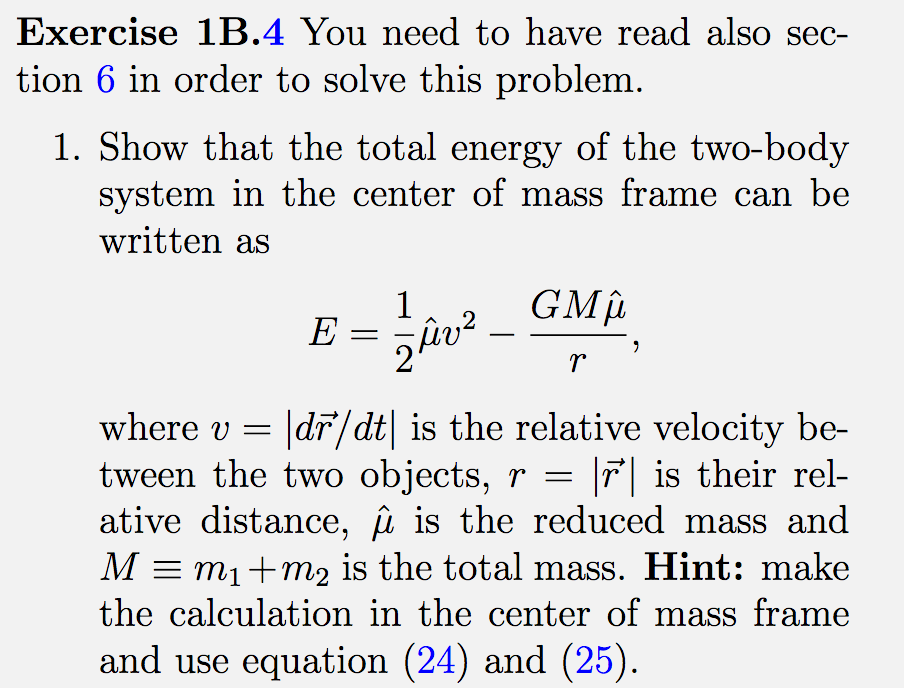
\includegraphics[scale=0.4]{media/1b4.png}\\
Ser du hvordan den kan løses?
Hvis ikke kan du få hjelp på gruppene.
Du trenger ikke gjøre det nå, men ta en titt på de neste to deloppgavene
\column{0.5\textwidth}
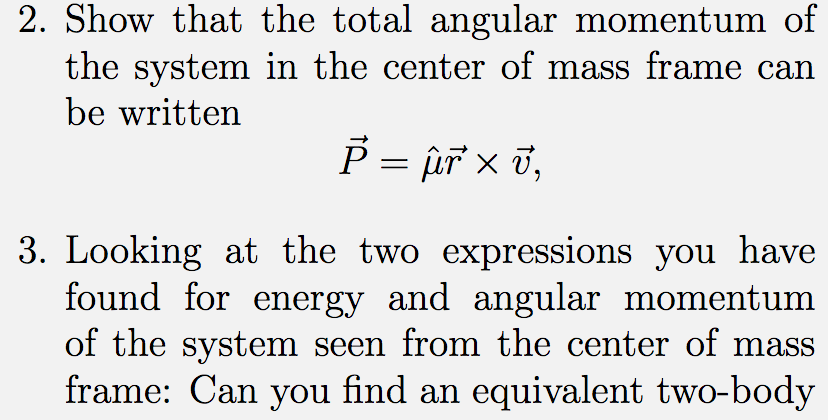
\includegraphics[scale=0.4]{media/1b4_2.png}\\
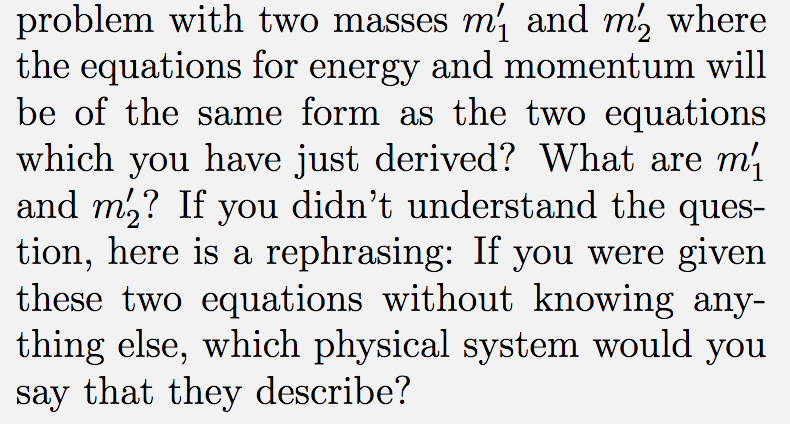
\includegraphics[scale=0.4]{media/1b4_3.png}\\
Hvis du sliter med å se hva som er svaret på tredje deloppgave, ta en titt på \href{https://www.uio.no/studier/emner/matnat/astro/AST2000/h20/undervisningsressurser/interaktive-forelesningsnotater/1b/videoer/video1b_13.mp4}{denne videoen}.
\hyperlink{energi5}{\pagebutton{Neste side}}
\end{columns}
\end{frame}


\begin{frame}
\label{energi5}
\lastpagebutton{energi4}
\addtocounter{pageno}{-1}
Men det vi var interessert i nå var å se hvordan energien kan avgjøre hvordan banen blir. For å gjøre det trenger vi først å repetere et par ting. Husker du hvordan vi fant hastighetsvektoren $\vec{v}$? Og husker du hva svaret var? (det bør du). Merk igjen, hastighetsvektoren $\vec{v}$ er den deriverte av posisjonsvektoren $\vec{r}$ som peker fra det ene legemet til det andre. Hastighetsvektoren $\vec{v}$ er dermed hastigheten til det ene legemet i forhold til det andre. Hvordan gjorde man nå det igjen? \hyperlink{energi5_b}{\pagebutton{Jeg husker/har repetert hvordan det var}}
\textcolor{white}{
\[
\vec{v}=\frac{d}{dt}\left(r\vec{e}_r\right)=\dot r\vec{e}_r+r\dot\theta\vec{e}_\theta
\]
Husker du hvorfor $v_\theta$ ser slik ut rent geometrisk? ({frisk opp!}).
Og så trenger vi en ting til, nemlig posisjonen $r(f)$ som funksjon av vinkel $f$ (hvordan var nå vinkelen $f$ definert?, det bør du repetere nå!).
\[
r=\frac{p}{1+e\cos{f}}
\]
hvor formen på $p$ og verdien på $e$ avgjør formen på banen.
{Neste side}}
\end{frame}


\begin{frame}
\label{energi5_b}
\lastpagebutton{energi4}
\addtocounter{pageno}{-1}
Men det vi var interessert i nå var å se hvordan energien kan avgjøre hvordan banen blir. For å gjøre det trenger vi først å repetere et par ting. Husker du hvordan vi fant hastighetsvektoren $\vec{v}$? Og husker du hva svaret var? (det bør du). Merk igjen, hastighetsvektoren $\vec{v}$ er den deriverte av posisjonsvektoren $\vec{r}$ som peker fra det ene legemet til det andre. Hastighetsvektoren $\vec{v}$ er dermed hastigheten til det ene legemet i forhold til det andre. Hvordan gjorde man nå det igjen? {\pagebutton{Jeg husker/har repetert hvordan det var}}
\[
\vec{v}=\frac{d}{dt}\left(r\vec{e}_r\right)=\dot r\vec{e}_r+r\dot\theta\vec{e}_\theta
\]
Husker du hvorfor $v_\theta$ ser slik ut rent geometrisk? (\href{https://www.uio.no/studier/emner/matnat/astro/AST2000/h20/undervisningsressurser/interaktive-forelesningsnotater/1b/videoer/video1b_3.mp4}{frisk opp!}).
Og så trenger vi en ting til, nemlig posisjonen $r(f)$ som funksjon av vinkel $f$ (hvordan var nå vinkelen $f$ definert?, det bør du repetere nå!).
\[
r=\frac{p}{1+e\cos{f}}
\]
hvor formen på $p$ og verdien på $e$ avgjør formen på banen.
\hyperlink{energi6}{\pagebutton{Neste side}}
\end{frame}






\begin{frame}
\label{energi6}
\dlastpagebutton{energi5}
Kjapp repetisjon før vi setter igang med utledningen som gir oss sammenheng mellom energi og baneformen:\\
Vi har
\[
r(f)=\frac{p}{1+e\cos{f}}
\]
der
\begin{itemize}
\item parabler har $e=1$ og $p=2a$
\item hyperbler har $e>1$ og $p=-a(1-e^2)$
\item ellipser har $e<1$ og $p=a(1-e^2)$
\end{itemize}
\hyperlink{energi7}{\pagebutton{Neste side}}
\end{frame}

\begin{frame}
\label{energi7}
\lastpagebutton{energi6}
Da har du alt du trenger for neste utledning som du finner \href{https://www.uio.no/studier/emner/matnat/astro/AST2000/h20/undervisningsressurser/interaktive-forelesningsnotater/1b/videoer/video1b_14.mp4}{i denne videoen her}. I videoen så kommer vi frem til følgende sammenheng mellom energi og $p$-en i uttrykket for $r$:
\[
E=\frac{\hat\mu m}{2p}(e^2-1)
\]
og husk igjen at $m=G(m_1+m_2)$. Her ser vi at hvis totalenergien er $E=0$, dvs. at den potensielle og kinetiske er like store med motsatt rettet fortegn, så {\bf må} $e=1$ på høyresiden. Dette tilsvarer en parabelbane (se forrige side). Hvis vi nå skriver om så har vi at:\\
\[
p=\frac{\hat\mu m}{2E}(e^2-1)
\]
Vi vet at $p$ må være en positiv størrelse (slik at $r$ er en positiv størrelse, se uttrykket for $r(f)$). Hvis energien $E$ her er positiv (kinetisk energi større enn potensiell), hva slags verdier kan $e$ ta for at $p$ blir positiv? Og hvis energien $E$ er negativ? (mer potensiell enn kinetisk) Hva slags verdier må $e$ da ta?\\
Tenk deg nøye om før du...
\hyperlink{energi8}{\pagebutton{... går videre til neste side}}
\end{frame}


\begin{frame}
\label{energi8}
\lastpagebutton{energi7}
Vi hadde
\[
p=\frac{\hat\mu m}{2E}(e^2-1)
\]
{\bf slik at hvis $E>0$ så må $e>1$ for at $p$ skal være positiv. Da får vi en hyperbelbane. Og hvis $E<0$ så få vi helt tilsvarende $e<1$ og vi har en ellipsebane.} Det gir mening siden ellipsebanen er bundet, og negativ energi betyr at potensiell gravitasjonsenergi 'vinner' over kinetisk energi. Og omvend for hyperbelbane, der 'vinner' den kinetiske energien og objektene er dermed ikke bundet som i hyperbelbanen. Vi ser også at parabelbanen er akkurat grensetilfellet mellom disse to.\textcolor{red}{ Hvordan finner vi så $a$ og $e$ til banen? Anta her en ellipsebane,} da har vi $p=a(1-e^2)$. Insatt i likningen gir det oss
\[
a=-\frac{\hat\mu m}{2E}
\]
At energien bestemmer hvor stor ellipsen er, har mening. \textcolor{blue}{Men hva med $e$? Det må vel ha noe med hastighetskomponentene å gjøre? Hvor mye hastighetene er rettet radielt eller tangensielt? Kan spinnet ha en rolle her?}
\hyperlink{energi9}{\pagebutton{Neste side}}
\end{frame}

\begin{frame}
\label{energi9}
\lastpagebutton{energi8}
I videoen på forrige side utledet vi et viktig mellomresultat:
\[
h=\sqrt{mp}
\]
en sammenheng mellom spinnet og $p$. Men her avhenger $p$ av $a$ som vi finner fra energien, samt eksentrisiteten $e$. Her overlates du til deg selv for å finne uttrykket for $e$ gitt at du kjenner spinnet til objektet.\\
Da har vi kommet til veis enda i dette kapittelet. Hvis du nå har en satelitt sin posisjon og hastighetskomponenter samt massen til satelitten og planeten så kan du øyeblikkelig beregne både formen på banen samt baneparameterene og fullstendig bestemme hvordan banen blir seende ut. Dette kommer du til å få bruk for i en del oppgaver, spesielt dere som tar prosjekt!
\hyperlink{skjema}{\pagebutton{Neste side}}
\end{frame}


\begin{frame}
\label{skjema}
\clastpagebuttonx{energi9}
{\Large
Før vi avslutter med litt tips og hjelp til koding av innleveringsoppgaven, må du teste/repetere at du har forstått stoffet vi har gått gjennom. Det gjør du på \href{https://nettskjema.no/a/155531}{dette skjemaet her}.
\hyperlink{koding}{\pagebutton{Ikke trykk her før skjemaet har blitt sendt inn}}
}
\end{frame}


\begin{frame}
\label{koding}
\begin{columns}
\column{0.5\textwidth}
{\small
\lastpagebuttonx{skjema}
\headlinebutton{\headline}\\
Men det blir også mye \textcolor{red}{numerisk baneberegning} som vi snakket om helt i starten av forrige forelesning mens \textcolor{blue}{de analytiske uttrykkene vi har utledet skal hjelpe oss med det numeriske.} Vi går tilbake til utgangspunktet vårt:
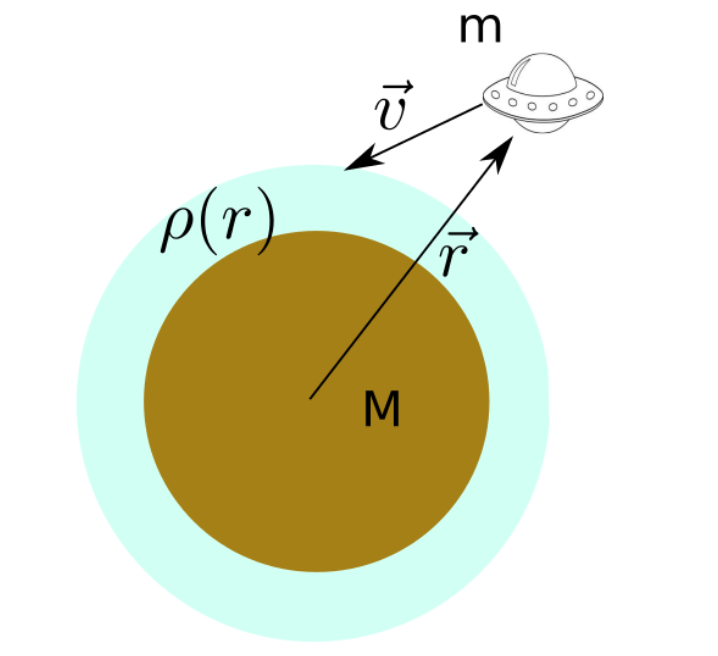
\includegraphics[scale=0.35]{media/landing.png}
Vi skal lande satelitten trygt. Her er det klart at du i den numeriske baneberegningen}
\column{0.5\textwidth}
{\small  også trenger å ta med friksjonskreftene når du kommer inn i atmosfæren. Dette er forklart nærmere i oppgave 1B8. Men når du å skal velge hvilken hastighet og retning du vil sende ut landersonden din ut fra modersonden med, gitt posisjonen din i banen, så har du nå fått god hjelp: ved å beregne energien og spinnet du får ved en gitt utgangshastighet så vet du nøyaktig hva slags bane du får. Kanskje strategien din er å lage en veldig avlang (eksentrisk) ellipsebane som sneier atmosfæren din ved hver nærpassering? Isåfall vet du nå hva du må gjøre med spinnet for å få en store $e$. Eller hvis du har en helt annen strategi: nå kan du forutsi hva slags bane du får frem til du begynner å treffe atmosfæren.}
\hyperlink{blue_nytema5}{\pagebutton{Neste side}}
\end{columns}
\end{frame}

\renewcommand{\headline}{\small Tips til koding}
{
\setbeamercolor{background canvas}{bg=blue}
\begin{frame}
\label{blue_nytema5}
\hyperlink{koding}{\pagebutton{\small Forrige side}}
\nytemaside{xxx}
\textcolor{yellow}{Som du nok har oppdaget så blir det alltid noen feil når man koder. Og det kan ta innmari lang tid å finne feilen. Dermed kommer igjen noen tips til feilsøking...}\\
\vspace*{0.5cm}
\hyperlink{koding2}{\pagebutton{Ja, kjekt å ha!}}
\end{frame}
}

\begin{frame}
\label{koding2}
\lastpagebutton{koding}
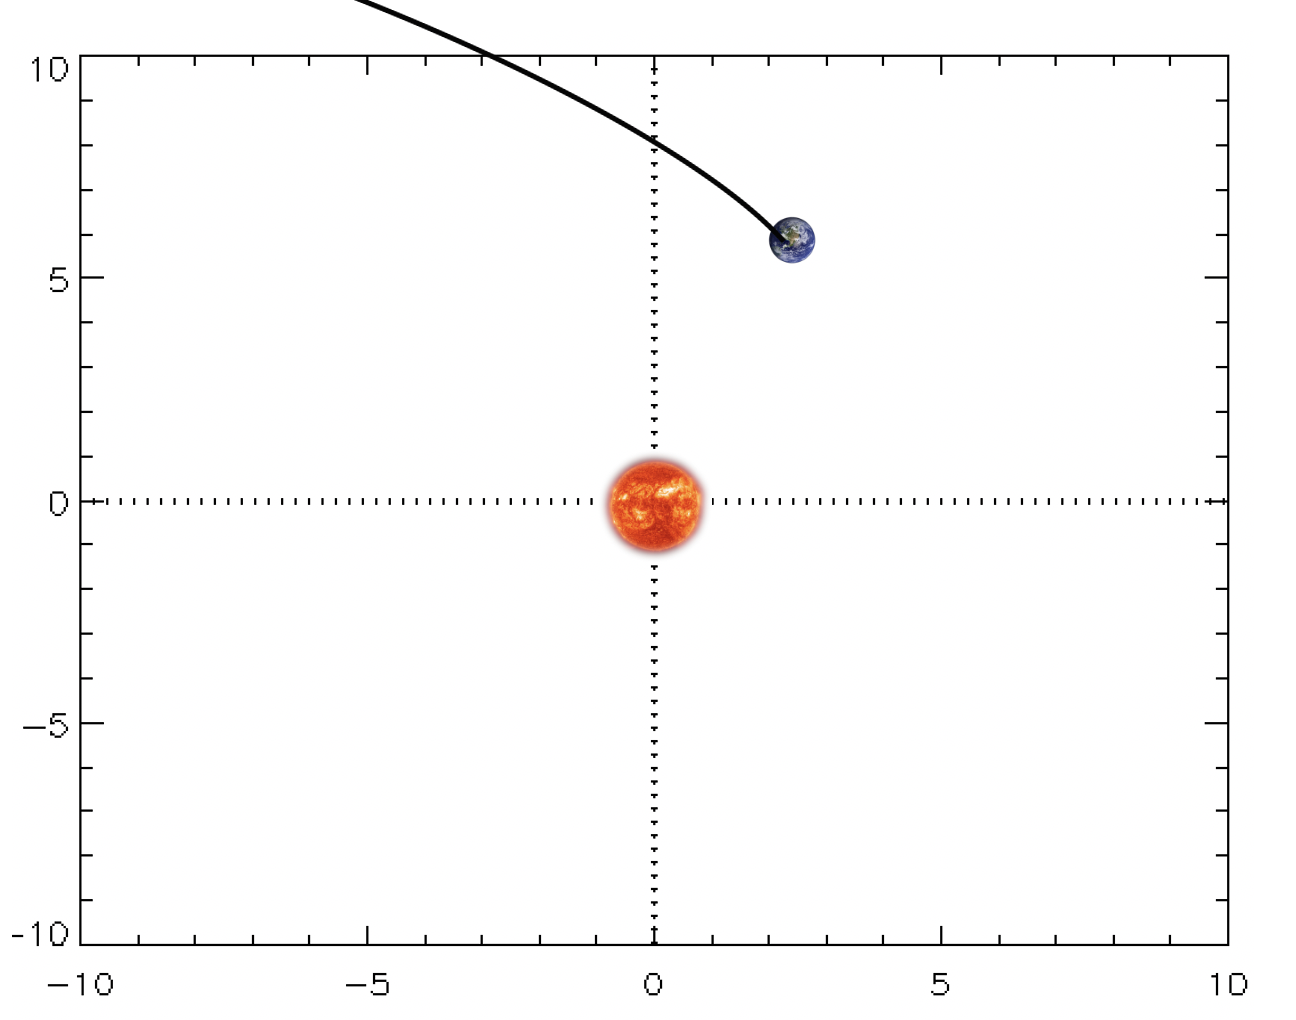
\includegraphics[scale=0.3]{media/debugging1.png}
{\small La oss helt til slutt snakke litt om debugging. Det kommer helt sikkert til å gå galt når du programmerer banen første gang. Her ser du et veldig typisk resultat (jordkloden indikerer startposisjon). \\{\bf Spørsmålet er, hva gjør du nå???}\\}
\hyperlink{feildebug}{\choicebutton{{\small Stirrer på koden til du finner feilen}}}\ \ \ \ \ \hyperlink{feildebug}{\choicebutton{{\small Får noen andre til å stirre på koden}}}\ \ \ \ \ \hyperlink{riktigdebug}{\choicebutton{{\small Bruker fysikk til å finne i hvilken del av koden feilen befinner seg.}}}
\end{frame}

{
\setbeamercolor{background canvas}{bg=black}
\begin{frame}
\label{feildebug}
\lastpagebutton{koding2}
\textcolor{white}{Det er en veldig god ide hvis du har masse fritid og liker å bruke laaaaaaaaang tid til å løse oppgaver.\\
Rådene på neste side er nok da ikke for deg, men \hyperlink{riktigdebug}{\pagebutton{Trykk her}} hvis du likevel har lyst til å få noen tips til hvordan du kan spare masse tid, så kan du jo bruke all tiden du har til overs på andre oppgaver?}
\end{frame}
}

{
\setbeamercolor{background canvas}{bg=yellow}
\begin{frame}
\label{riktigdebug}
\begin{columns}
\column{0.5\textwidth}
\clastpagebuttonx{koding2}
\headlinebutton{\headline}\\
{\small Det er en utmerket ide å bruke litt fysikk når man gjør debugging, husk dette også for de kommende delene i kurset. Du kan spare {\bf masse} tid på debugging hvis du bare finner ut hvor feilen ligger. La oss se på noen mulige strategier i dette tilfellet her.\\}
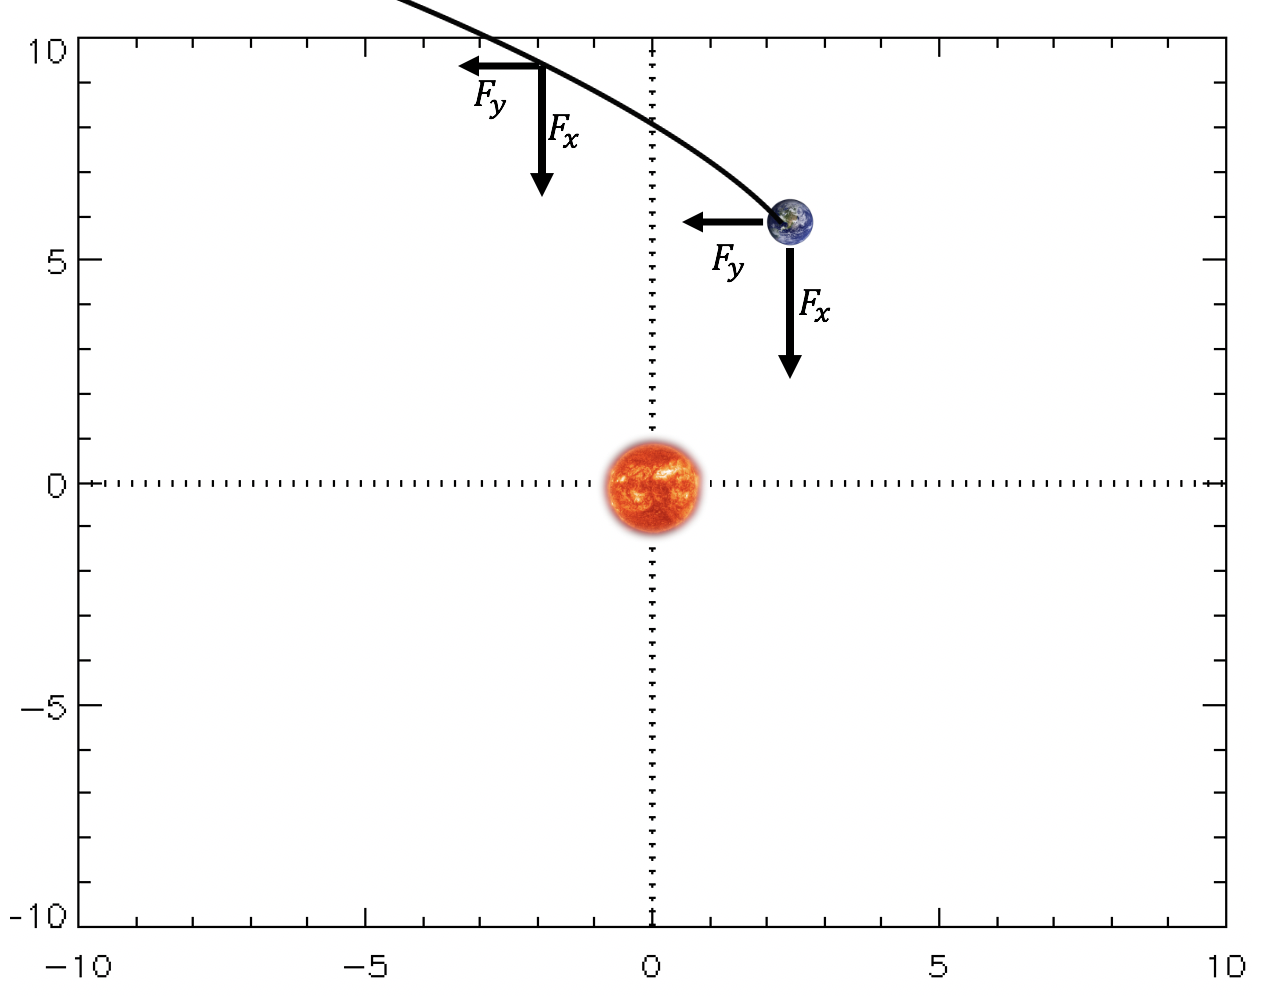
\includegraphics[scale=0.3]{media/debugging2.png}\\
\column{0.5\textwidth}
\begin{enumerate}
\item Hva er energien din i initialposisjonen? Er $E>0$? Da er det enten noe feil med initialhastigheten din, eller du skal ha en hyperbelbane.
\item Lag en liste med energien i hvert tidssteg. Endrer energien seg? (det skal den ikke hvis du kun har gravitasjonskraft)
\item Hvis energien endrer seg må kraften være gal. Sjekk komponentene $F_x$ og $F_y$. Peker de riktig, dvs. har de riktig fortegn? (se figur)
\item Sjekk kraft-komponentene både i initialposisjonen og noen tidssteg senere (se figur)
\end{enumerate}
\hyperlink{koding3}{\pagebutton{Neste side}}
\end{columns}
\end{frame}
}

\begin{frame}
\label{koding3}
\begin{columns}
\column{0.5\textwidth}
\lastpagebutton{riktigdebug}
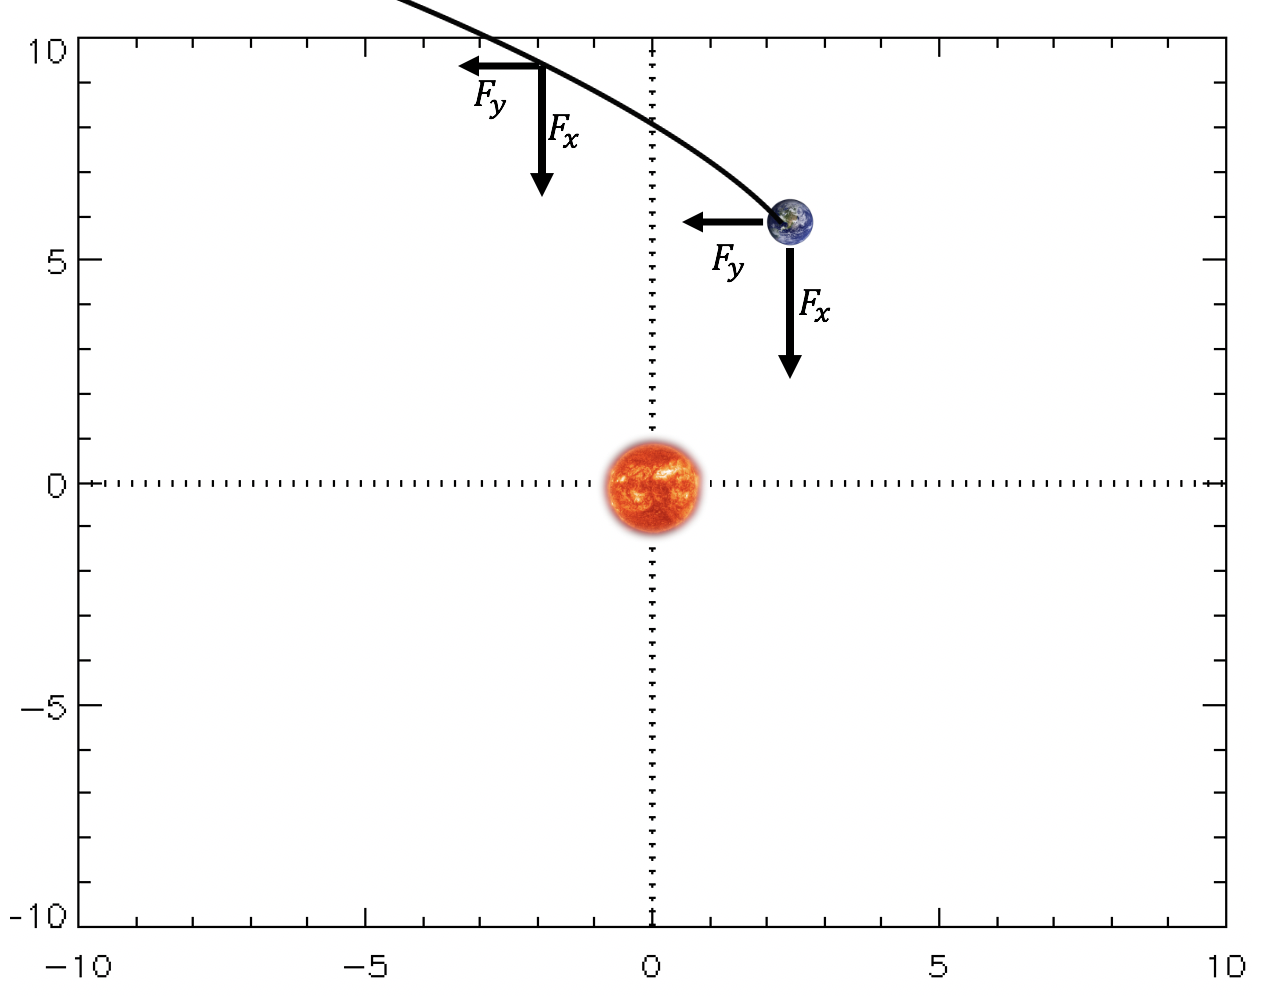
\includegraphics[scale=0.25]{media/debugging2.png}
{\small
{\bf Og sist, men ikke minst:} Sjekk størrelsen på kraftvektoren. {\bf Bruk kalkulator (dette er viktig slik at du bruker noe helt annet en koden din)} til å beregne totalkrafta i initialposisjonen. Beregn først lengden av initialposisjonsvektoren $\vec{r}$ {\bf (også med kalkulator)} og så størrelsen på krafta.} 
\column{0.5\textwidth}
\\
{\small Sammenlikn krafta med det du finner i koden (absoluttverdi av kraftvektoren). Er den feil, sjekk også om du har beregnet lengden av posisjonsvektoren riktig. Hvis alt er riktig, gjenta dette en del tidssteg senere, er krafta enda riktig? Her vil du veldig ofte finne at du beregner krafta feil i koden. Iblant kan det være vanskelig å ovrersette formler riktig til python, derfor er denne uavhengige kontrollen på papir/kalkulator veldig viktig.}\\
{\bf\large Følger du prosedyren på denne og foregående side så er det nesten helt sikkert at du klarer å finne feilen selv!\\}
 \hyperlink{oppsummering}{\pagebutton{Neste side}}
\end{columns}
\end{frame}


\begin{frame}
\label{oppsummering}
\hyperlink{koding3}{\pagebutton{\small Forrige side}}\href{https://nettskjema.no/a/158672}{\Changey[1][yellow]{2} \Changey[1][yellow]{-2}}
Gratulerer, da er del 1B overstått! Du bør nå kunne:
\begin{itemize}
\item beskrive de forskjellige banene som er løsninger av to-legeme-problemet
\item kunne beregne slike baner både analytisk og numerisk
\item vite hvilke parametere som beskriver slike baner og vite hvordan finne slike parametere
\item kunne regne med Newtons lover på vektorform 
\item og dermed kunne regne med posisjosvektorer, hastighetsvektorer og kraftvektorer dekomponert både i kartesiske enhetsvektorer men også i radielle og tangensielle enhetsvektorer
\item kunne beskrive og beregne på baner i et tolegemesystem sett fra massesentersystemet
\item kunne beregne anguklærmoment og energi i et slikt to-legemesystem
\end{itemize}
    {\bf\footnotesize Det anbefales nå at du sjekker \href{https://www.uio.no/studier/emner/matnat/astro/AST2000/h21/undervisningsmateriell/kortsvarsoppgaver/del1b.pdf}{kortsvarsoppgavene} til del 1B for å kontrollere at du har forstått stoffet. Kan du svare på disse, blir det lettere å bruke kunnskapen din i oppgavene/prosjektet. Noen av disse kommer på eksamen.}
\textcolor{red}{\footnotesize Trykk nå gjerne på smilefjesene og si meninga di om dette interaktive forelesningsnotatet. Spesielt er jeg interessert i å vite hvor lang tid du brukte og da hva du brukte mest tid på! All ris og ros mottaes med takk.}
\end{frame}

\end{document}
